\documentclass{report}

%%METADATA
\title{Logbook for Fall 2020 Independent Study}
\author{
Luke Motley
}
\date{}

%%PACKAGES
\usepackage{graphicx}
\usepackage{tabularx}
\usepackage{setspace}
\usepackage{amsmath,amsthm,amssymb}
\usepackage[hyphens]{url}
\usepackage{natbib}
\usepackage[font=normalsize,labelfont=bf]{caption}
\usepackage[margin=1in]{geometry}
\usepackage{hyperref}
\hypersetup{colorlinks=true,urlcolor=blue,citecolor=red}
\usepackage{enumerate}% http://ctan.org/pkg/enumerate %Supports lowercase Roman-letter enumeration
\usepackage{verbatim} %Package with \begin{comment} environment
\usepackage{physics}
\usepackage{lscape}
\usepackage{tikz}
\usepackage{tikz-3dplot}
\usepackage{tkz-euclide}
\usepackage{pgfplots}
\pgfplotsset{compat = newest}
\usetikzlibrary{automata,positioning}
\usepgfplotslibrary{external}
\tikzexternalize
\usetikzlibrary{calc,math}
\usepackage{listings}
\usepackage{ulem}
\usepackage{upquote}
\usepackage{booktabs} %Package with \toprule and \bottomrule
\usepackage{etoc}     %Package with \localtableofcontents
\usepackage{multicol}
\usepackage{bm}
\usepackage{placeins} %Package with \FloatBarrier
\setlength{\parskip}{0.5em}
\usepackage{subcaption}
\captionsetup{compatibility=false}


\definecolor{dkgreen}{rgb}{0,0.6,0}
\definecolor{gray}{rgb}{0.5,0.5,0.5}
\definecolor{mauve}{rgb}{0.58,0,0.82}

\lstset{language=bash,
  frame=tb,
  aboveskip=3mm,
  belowskip=3mm,
  showstringspaces=false,
  columns=flexible,
  basicstyle={\small\ttfamily},
  numbers=none,
  numberstyle=\tiny\color{gray},
  keywordstyle=\color{blue},
  commentstyle=\color{dkgreen},
  stringstyle=\color{mauve},
  breaklines=true,
  breakatwhitespace=false,
  tabsize=3
}

% ---------------------------------------------------------------------
% Program: listings-stata.tex
% Author:  github.com/mcaceresb
% Purpose: Stata language definition for LaTeX listings package
% Usage:   Add % ---------------------------------------------------------------------
% Program: listings-stata.tex
% Author:  github.com/mcaceresb
% Purpose: Stata language definition for LaTeX listings package
% Usage:   Add % ---------------------------------------------------------------------
% Program: listings-stata.tex
% Author:  github.com/mcaceresb
% Purpose: Stata language definition for LaTeX listings package
% Usage:   Add \input{listings-stata.tex} to your preamble

% Syntax from
% - https://github.com/isagalaev/highlight.js/blob/master/src/languages/stata.js
% - https://github.com/jpitblado/vim-stata/blob/master/syntax/stata.vim
% - http://fmwww.bc.edu/RePEc/bocode/s/synlightlist.ado

\RequirePackage{listings}
\RequirePackage{color}
%\RequirePackage[svgnames]{xcolor}
%\definecolor{spRed}{HTML}{BE646C}

% ---------------------------------------------------------------------
% Stata language definition

\lstdefinelanguage{stata}{
  sensitive=true,
  %
  % Macros, global and local
  alsoletter={\{\}0123456789},
  keywordsprefix=\$,
  morecomment=[n][keywordstyle9]{`}{'},
  morekeywords={},
  %
  % Comments
  morecomment=[f][\color{Green}\slshape][0]*,
  morecomment=[l]{//},
  morecomment=[s]{/*}{*/},
  %
  % Strings
  morecomment=[n][\color{Maroon}]{`"}{"'},
  morestring=[b]",
  %
  % Add-ons and system Commands
  morekeywords=[2]{
    if ,else ,in ,foreach ,for ,forv ,forva ,forval ,forvalu ,forvalue
    ,forvalues ,by ,bys ,bysort ,xi ,quietly ,qui ,capture ,about
    ,ac ,ac_7 ,acprplot ,acprplot_7 adjust ,ado ,adopath ,adoupdate
    ,alpha ,ameans ,an ,ano ,anov ,anova ,anova_estat ,anova_terms
    ,anovadef ,aorder ,ap ,app ,appe ,appen ,append ,arch ,arch_dr
    ,arch_estat ,arch_p ,archlm ,areg ,areg_p ,args ,arima ,arima_dr
    ,arima_estat ,arima_p ,as ,asmprobit ,asmprobit_estat ,asmprobit_lf
    ,asmprobit_mfx__dlg ,asmprobit_p ,ass ,asse ,asser ,assert ,avplot
    ,avplot_7 ,avplots ,avplots_7 bcskew0 ,bgodfrey ,binreg ,bip0_lf
    ,biplot ,bipp_lf ,bipr_lf ,bipr_p ,biprobit ,bitest ,bitesti
    ,bitowt ,blogit ,bmemsize ,boot ,bootsamp ,bootstrap ,bootstrap_8
    ,boxco_l ,boxco_p ,boxcox ,boxcox_6 ,boxcox_p ,bprobit ,br ,break
    ,brier ,bro ,brow ,brows ,browse ,brr ,brrstat ,bs ,bs_7 ,bsampl_w
    ,bsample ,bsample_7 ,bsqreg ,bstat ,bstat_7 ,bstat_8 ,bstrap
    ,bstrap_7 ,ca ,ca_estat ,ca_p ,cabiplot ,camat ,canon ,canon_8
    ,canon_8_p ,canon_estat ,canon_p ,cap ,caprojection ,capt ,captu
    ,captur ,capture ,cat ,cc ,cchart ,cchart_7 ,cci ,cd ,censobs_table
    ,centile ,cf ,char ,chdir ,checkdlgfiles ,checkestimationsample
    ,checkhlpfiles ,checksum ,chelp ,ci ,cii ,cl ,class ,classutil
    ,clear ,cli ,clis ,clist ,clo ,clog ,clog_lf ,clog_p ,clogi
    ,clogi_sw ,clogit ,clogit_lf ,clogit_p ,clogitp ,clogl_sw ,cloglog
    ,clonevar ,clslistarray ,cluster ,cluster_measures ,cluster_stop
    ,cluster_tree ,cluster_tree_8 ,clustermat ,cmdlog ,cnr ,cnre
    ,cnreg ,cnreg_p ,cnreg_sw ,cnsreg ,codebook ,collaps4 ,collapse
    ,colormult_nb ,colormult_nw ,compare ,compress ,conf ,confi
    ,confir ,confirm ,conren ,cons ,const ,constr ,constra ,constrai
    ,constrain ,constraint ,continue ,contract ,copy ,copyright
    ,copysource ,cor ,corc ,corr ,corr2data ,corr_anti ,corr_kmo
    ,corr_smc ,corre ,correl ,correla ,correlat ,correlate ,corrgram
    ,cou ,coun ,count ,cox ,cox_p ,cox_sw ,coxbase ,coxhaz ,coxvar
    ,cprplot ,cprplot_7 ,crc ,cret ,cretu ,cretur ,creturn ,cross ,cs
    ,cscript ,cscript_log ,csi ,ct ,ct_is ,ctset ,ctst_5 ,ctst_st
    ,cttost ,cumsp ,cumsp_7 ,cumul ,cusum ,cusum_7 ,cutil ,d ,datasig
    ,datasign ,datasigna ,datasignat ,datasignatu ,datasignatur
    ,datasignature ,datetof ,db ,dbeta ,de ,dec ,deco ,decod ,decode
    ,deff ,des ,desc ,descr ,descri ,describ ,describe ,destring
    ,dfbeta ,dfgls ,dfuller ,di ,di_g ,dir ,dirstats ,dis ,discard
    ,disp ,disp_res ,disp_s ,displ ,displa ,display ,distinct ,do
    ,doe ,doed ,doedi ,doedit ,dotplot ,dotplot_7 ,dprobit ,drawnorm
    ,drop ,ds ,ds_util ,dstdize ,duplicates ,durbina ,dwstat ,dydx ,e
    ,ed ,edi ,edit ,egen ,eivreg ,emdef ,en ,enc ,enco ,encod ,encode
    ,eq ,erase ,ereg ,ereg_lf ,ereg_p ,ereg_sw ,ereghet ,ereghet_glf
    ,ereghet_glf_sh ,ereghet_gp ,ereghet_ilf ,ereghet_ilf_sh ,ereghet_ip
    ,eret ,eretu ,eretur ,ereturn ,err ,erro ,error ,est ,est_cfexist
    ,est_cfname ,est_clickable ,est_expand ,est_hold ,est_table
    ,est_unhold ,est_unholdok ,estat ,estat_default ,estat_summ
    ,estat_vce_only ,esti ,estimates ,etodow ,etof ,etomdy ,ex ,exi
    ,exit ,expand ,expandcl ,fac ,fact ,facto ,factor ,factor_estat
    ,factor_p ,factor_pca_rotated ,factor_rotate ,factormat ,fcast
    ,fcast_compute ,fcast_graph ,fdades ,fdadesc ,fdadescr ,fdadescri
    ,fdadescrib ,fdadescribe ,fdasav ,fdasave ,fdause ,fh_st ,file
    ,open ,file ,read ,file ,close ,file ,filefilter ,fillin
    ,find_hlp_file ,findfile ,findit ,findit_7 ,fit ,fl ,fli ,flis
    ,flist ,for5_0 ,form ,forma ,format ,fpredict ,frac_154 ,frac_adj
    ,frac_chk ,frac_cox ,frac_ddp ,frac_dis ,frac_dv ,frac_in ,frac_mun
    ,frac_pp ,frac_pq ,frac_pv ,frac_wgt ,frac_xo ,fracgen ,fracplot
    ,fracplot_7 ,fracpoly ,fracpred ,fron_ex ,fron_hn ,fron_p ,fron_tn
    ,fron_tn2 ,frontier ,ftodate ,ftoe ,ftomdy ,ftowdate ,g ,gamhet_glf
    ,gamhet_gp ,gamhet_ilf ,gamhet_ip ,gamma ,gamma_d2 ,gamma_p
    ,gamma_sw ,gammahet ,gdi_hexagon ,gdi_spokes ,ge ,gen ,gene ,gener
    ,genera ,generat ,generate ,genrank ,genstd ,genvmean ,gettoken
    ,gl ,gladder ,gladder_7 ,glim_l01 ,glim_l02 glim_l03 ,glim_l04
    ,glim_l05 ,glim_l06 ,glim_l07 ,glim_l08 ,glim_l09 ,glim_l10 glim_l11
    ,glim_l12 ,glim_lf ,glim_mu ,glim_nw1 ,glim_nw2 ,glim_nw3 ,glim_p
    ,glim_v1 ,glim_v2 ,glim_v3 ,glim_v4 ,glim_v5 ,glim_v6 ,glim_v7 ,glm
    ,glm_6 glm_p ,glm_sw ,glmpred ,glo ,glob ,globa ,global ,glogit
    ,glogit_8 ,glogit_p ,gmeans ,gnbre_lf ,gnbreg ,gnbreg_5 ,gnbreg_p
    ,gomp_lf ,gompe_sw ,gomper_p ,gompertz ,gompertzhet ,gomphet_glf
    ,gomphet_glf_sh ,gomphet_gp ,gomphet_ilf ,gomphet_ilf_sh ,gomphet_ip
    ,gphdot ,gphpen ,gphprint ,gprefs ,gprobi_p ,gprobit ,gprobit_8
    ,gr ,gr7 ,gr_copy ,gr_current ,gr_db ,gr_describe ,gr_dir ,gr_draw
    ,gr_draw_replay ,gr_drop ,gr_edit ,gr_editviewopts ,gr_example
    ,gr_example2 gr_export ,gr_print ,gr_qscheme ,gr_query ,gr_read
    ,gr_rename ,gr_replay ,gr_save ,gr_set ,gr_setscheme ,gr_table
    ,gr_undo ,gr_use ,graph ,graph7 grebar ,greigen ,greigen_7
    ,greigen_8 ,grmeanby ,grmeanby_7 ,gs_fileinfo ,gs_filetype
    ,gs_graphinfo ,gs_stat ,gsort ,gwood ,h ,hadimvo ,hareg ,hausman
    ,haver ,he ,heck_d2 ,heckma_p ,heckman ,heckp_lf ,heckpr_p ,heckprob
    ,hel ,help ,hereg ,hetpr_lf ,hetpr_p ,hetprob ,hettest ,hexdump
    ,hilite ,hist ,hist_7 histogram ,hlogit ,hlu ,hmeans ,hotel
    ,hotelling ,hprobit ,hreg ,hsearch ,icd9 ,icd9_ff ,icd9p ,iis
    ,impute ,imtest ,inbase ,include ,inf ,infi ,infil ,infile ,infix
    ,inp ,inpu ,input ,ins ,insheet ,insp ,inspe ,inspec ,inspect ,integ
    ,inten ,intreg ,intreg_7 ,intreg_p ,intrg2_ll ,intrg_ll ,intrg_ll2
    ,ipolate ,iqreg ,ir ,irf ,irf_create ,irfm ,iri ,is_svy ,is_svysum
    ,isid ,istdize ,ivprob_1_lf ,ivprob_lf ,ivprobit ,ivprobit_p ,ivreg
    ,ivreg_footnote ,ivtob_1_lf ,ivtob_lf ,ivtobit ,ivtobit_p ,jackknife
    ,jacknife ,jknife ,jknife_6 ,jknife_8 ,jkstat ,joinby ,kalarma1
    ,kap ,kap_3 ,kapmeier ,kappa ,kapwgt ,kdensity ,kdensity_7 keep
    ,ksm ,ksmirnov ,ktau ,kwallis ,l ,la ,lab ,labe ,label ,labelbook
    ,ladder ,levels ,levelsof ,leverage ,lfit ,lfit_p ,li ,lincom ,line
    ,linktest ,lis ,list ,lloghet_glf ,lloghet_glf_sh ,lloghet_gp
    ,lloghet_ilf ,lloghet_ilf_sh ,lloghet_ip ,llogi_sw ,llogis_p
    ,llogist ,llogistic ,llogistichet ,lnorm_lf ,lnorm_sw ,lnorma_p
    ,lnormal ,lnormalhet ,lnormhet_glf ,lnormhet_glf_sh ,lnormhet_gp
    ,lnormhet_ilf ,lnormhet_ilf_sh ,lnormhet_ip ,lnskew0 ,loadingplot
    ,loc ,loca ,local ,log ,logi ,logis_lf ,logistic ,logistic_p
    ,logit ,logit_estat ,logit_p ,loglogs ,logrank ,loneway ,lookfor
    ,lookup ,lowess ,lowess_7 ,lpredict ,lrecomp ,lroc ,lroc_7 ,lrtest
    ,ls ,lsens ,lsens_7 ,lsens_x ,lstat ,ltable ,ltable_7 ,ltriang
    ,lv ,lvr2plot ,lvr2plot_7 ,m ,ma ,mac ,macr ,macro ,makecns ,man
    ,manova ,manova_estat ,manova_p ,manovatest ,mantel ,mark ,markin
    ,markout ,marksample ,mat ,mat_capp ,mat_order ,mat_put_rr ,mat_rapp
    ,mata ,mata_clear ,mata_describe ,mata_drop ,mata_matdescribe
    ,mata_matsave ,mata_matuse ,mata_memory ,mata_mlib ,mata_mosave
    ,mata_rename ,mata_which ,matalabel ,matcproc ,matlist ,matname
    ,matr ,matri ,matrix ,matrix_input__dlg ,matstrik ,mcc ,mcci ,md0_
    ,md1_ ,md1debug_ ,md2_ ,md2debug_ ,mds ,mds_estat ,mds_p ,mdsconfig
    ,mdslong ,mdsmat ,mdsshepard ,mdytoe ,mdytof ,me_derd ,mean ,means
    ,median ,memory ,memsize ,meqparse ,mer ,merg ,merge ,mfp ,mfx
    ,mhelp ,mhodds ,minbound ,mixed_ll ,mixed_ll_reparm ,mkassert
    ,mkdir ,mkmat ,mkspline ,ml ,ml_5 ml_adjs ,ml_bhhhs ,ml_c_d
    ,ml_check ,ml_clear ,ml_cnt ,ml_debug ,ml_defd ,ml_e0 ml_e0_bfgs
    ,ml_e0_cycle ,ml_e0_dfp ,ml_e0i ,ml_e1 ,ml_e1_bfgs ,ml_e1_bhhh
    ,ml_e1_cycle ,ml_e1_dfp ,ml_e2 ,ml_e2_cycle ,ml_ebfg0 ,ml_ebfr0
    ,ml_ebfr1 ml_ebh0q ,ml_ebhh0 ,ml_ebhr0 ,ml_ebr0i ,ml_ecr0i ,ml_edfp0
    ,ml_edfr0 ,ml_edfr1 ml_edr0i ,ml_eds ,ml_eer0i ,ml_egr0i ,ml_elf
    ,ml_elf_bfgs ,ml_elf_bhhh ,ml_elf_cycle ,ml_elf_dfp ,ml_elfi
    ,ml_elfs ,ml_enr0i ,ml_enrr0 ,ml_erdu0 ml_erdu0_bfgs ,ml_erdu0_bhhh
    ,ml_erdu0_bhhhq ,ml_erdu0_cycle ,ml_erdu0_dfp ,ml_erdu0_nrbfgs
    ,ml_exde ,ml_footnote ,ml_geqnr ,ml_grad0 ,ml_graph ,ml_hbhhh
    ,ml_hd0 ,ml_hold ,ml_init ,ml_inv ,ml_log ,ml_max ,ml_mlout
    ,ml_mlout_8 ,ml_model ,ml_nb0 ,ml_opt ,ml_p ,ml_plot ,ml_query
    ,ml_rdgrd ,ml_repor ,ml_s_e ,ml_score ,ml_searc ,ml_technique
    ,ml_unhold ,mleval ,mlf_ ,mlmatbysum ,mlmatsum ,mlog ,mlogi ,mlogit
    ,mlogit_footnote ,mlogit_p ,mlopts ,mlsum ,mlvecsum ,mnl0_ ,mor
    ,more ,mov ,move ,mprobit ,mprobit_lf ,mprobit_p ,mrdu0_ ,mrdu1_
    ,mvdecode ,mvencode ,mvreg ,mvreg_estat ,n ,nbreg ,nbreg_al
    ,nbreg_lf ,nbreg_p ,nbreg_sw ,nestreg ,net ,newey ,newey_7 ,newey_p
    ,news ,nl ,nl_7 ,nl_9 ,nl_9_p ,nl_p ,nl_p_7 nlcom ,nlcom_p ,nlexp2
    ,nlexp2_7 ,nlexp2a ,nlexp2a_7 ,nlexp3 ,nlexp3_7 ,nlgom3 nlgom3_7
    ,nlgom4 ,nlgom4_7 ,nlinit ,nllog3 ,nllog3_7 ,nllog4 ,nllog4_7
    ,nlog_rd ,nlogit ,nlogit_p ,nlogitgen ,nlogittree ,nlpred ,no
    ,nobreak ,noi ,nois ,noisi ,noisil ,noisily ,note ,notes ,notes_dlg
    ,nptrend ,numlabel ,numlist ,odbc ,old_ver ,olo ,olog ,ologi
    ,ologi_sw ,ologit ,ologit_p ,ologitp ,on ,one ,onew ,onewa ,oneway
    ,op_colnm ,op_comp ,op_diff ,op_inv ,op_str ,opr ,opro ,oprob
    ,oprob_sw ,oprobi ,oprobi_p ,oprobit ,oprobitp ,opts_exclusive
    ,order ,orthog ,orthpoly ,ou ,out ,outf ,outfi ,outfil ,outfile
    ,outs ,outsh ,outshe ,outshee ,outsheet ,ovtest ,pac ,pac_7 ,palette
    ,parse ,parse_dissim ,pause ,pca ,pca_8 pca_display ,pca_estat
    ,pca_p ,pca_rotate ,pcamat ,pchart ,pchart_7 ,pchi ,pchi_7 ,pcorr
    ,pctile ,pentium ,pergram ,pergram_7 ,permute ,permute_8 ,personal
    ,peto_st ,pkcollapse ,pkcross ,pkequiv ,pkexamine ,pkexamine_7
    ,pkshape ,pksumm ,pksumm_7 ,pl ,plo ,plot ,plugin ,pnorm ,pnorm_7
    ,poisgof ,poiss_lf ,poiss_sw ,poisso_p ,poisson ,poisson_estat
    ,post ,postclose ,postfile ,postutil ,pperron ,pr ,prais ,prais_e
    ,prais_e2 ,prais_p ,predict ,predictnl ,preserve ,print ,pro ,prob
    ,probi ,probit ,probit_estat ,probit_p ,proc_time ,procoverlay
    ,procrustes ,procrustes_estat ,procrustes_p ,profiler ,prog ,progr
    ,progra ,program ,prop ,proportion ,prtest ,prtesti ,pwcorr ,pwd
    ,q ,s ,qby ,qbys ,qchi ,qchi_7 ,qladder ,qladder_7 ,qnorm ,qnorm_7
    ,qqplot ,qqplot_7 ,qreg ,qreg_c ,qreg_p ,qreg_sw ,qu ,quadchk
    ,quantile ,quantile_7 ,que ,quer ,query ,range ,ranksum ,ratio
    ,rchart ,rchart_7 ,rcof ,recast ,reclink ,recode ,reg ,reg3
    ,reg3_p ,regdw ,regr ,regre ,regre_p2 ,regres ,regres_p ,regress
    ,regress_estat ,regriv_p ,remap ,ren ,rena ,renam ,rename ,renpfix
    ,repeat ,replace ,report ,reshape ,restore ,ret ,retu ,retur ,return
    ,rm ,rmdir ,robvar ,roccomp ,roccomp_7 ,roccomp_8 ,rocf_lf ,rocfit
    ,rocfit_8 ,rocgold ,rocplot ,rocplot_7 ,roctab ,roctab_7 ,rolling
    ,rologit ,rologit_p ,rot ,rota ,rotat ,rotate ,rotatemat ,rreg
    ,rreg_p ,ru ,run ,runtest ,rvfplot ,rvfplot_7 ,rvpplot ,rvpplot_7
    ,sa ,safesum ,sample ,sampsi ,sav ,save ,savedresults ,saveold ,sc
    ,sca ,scal ,scala ,scalar ,scatter ,scm_mine ,sco ,scob_lf ,scob_p
    ,scobi_sw ,scobit ,scor ,score ,scoreplot ,scoreplot_help ,scree
    ,screeplot ,screeplot_help ,sdtest ,sdtesti ,se ,search ,separate
    ,seperate ,serrbar ,serrbar_7 ,serset ,set ,set_defaults ,sfrancia
    ,sh ,she ,shel ,shell ,shewhart ,shewhart_7 ,signestimationsample
    ,signrank ,signtest ,simul ,simul_7 simulate ,simulate_8 ,sktest
    ,sleep ,slogit ,slogit_d2 ,slogit_p ,smooth ,snapspan ,so ,sor
    ,sort ,spearman ,spikeplot ,spikeplot_7 ,spikeplt ,spline_x ,split
    ,sqreg ,sqreg_p ,sret ,sretu ,sretur ,sreturn ,ssc ,st ,st_ct ,st_hc
    ,st_hcd ,st_hcd_sh ,st_is ,st_issys ,st_note ,st_promo ,st_set
    ,st_show ,st_smpl ,st_subid ,stack ,statsby ,statsby_8 ,stbase
    ,stci ,stci_7 ,stcox ,stcox_estat ,stcox_fr ,stcox_fr_ll ,stcox_p
    ,stcox_sw ,stcoxkm ,stcoxkm_7 ,stcstat ,stcurv ,stcurve ,stcurve_7
    ,stdes ,stem ,stepwise ,stereg ,stfill ,stgen ,stir ,stjoin ,stmc
    ,stmh ,stphplot ,stphplot_7 ,stphtest ,stphtest_7 ,stptime ,strate
    ,strate_7 ,streg ,streg_sw ,streset ,sts ,sts_7 ,stset ,stsplit
    ,stsum ,sttocc ,sttoct ,stvary ,stweib ,su ,suest ,suest_8 ,sum
    ,summ ,summa ,summar ,summari ,summariz ,summarize ,sunflower
    ,sureg ,survcurv ,survsum ,svar ,svar_p ,svmat ,svy ,svy_disp
    ,svy_dreg ,svy_est ,svy_est_7 ,svy_estat ,svy_get ,svy_gnbreg_p
    ,svy_head ,svy_header ,svy_heckman_p ,svy_heckprob_p ,svy_intreg_p
    ,svy_ivreg_p ,svy_logistic_p ,svy_logit_p ,svy_mlogit_p ,svy_nbreg_p
    ,svy_ologit_p ,svy_oprobit_p ,svy_poisson_p ,svy_probit_p
    ,svy_regress_p ,svy_sub ,svy_sub_7 ,svy_x ,svy_x_7 ,svy_x_p ,svydes
    ,svydes_8 ,svygen ,svygnbreg ,svyheckman ,svyheckprob ,svyintreg
    ,svyintreg_7 ,svyintrg ,svyivreg ,svylc ,svylog_p ,svylogit
    ,svymarkout ,svymarkout_8 ,svymean ,svymlog ,svymlogit ,svynbreg
    ,svyolog ,svyologit ,svyoprob ,svyoprobit ,svyopts ,svypois
    ,svypois_7 svypoisson ,svyprobit ,svyprobt ,svyprop ,svyprop_7
    ,svyratio ,svyreg ,svyreg_p ,svyregress ,svyset ,svyset_7 ,svyset_8
    ,svytab ,svytab_7 ,svytest ,svytotal ,sw ,sw_8 ,swcnreg ,swcox
    ,swereg ,swilk ,swlogis ,swlogit ,swologit ,swoprbt ,swpois
    ,swprobit ,swqreg ,swtobit ,swweib ,symmetry ,symmi ,symplot
    ,symplot_7 syntax ,sysdescribe ,sysdir ,sysuse ,szroeter ,ta ,tab
    ,tab1 ,tab2 ,tab_or ,tabd ,tabdi ,tabdis ,tabdisp ,tabi ,table
    ,tabodds ,tabodds_7 ,tabstat ,tabu ,tabul ,tabula ,tabulat ,tabulate
    ,te ,tempfile ,tempname ,tempvar ,tes ,test ,testnl ,testparm
    ,teststd ,tetrachoric ,time_it ,timer ,tis ,tob ,tobi ,tobit
    ,tobit_p ,tobit_sw ,token ,tokeni ,tokeniz ,tokenize ,tostring
    ,total ,translate ,translator ,transmap ,treat_ll ,treatr_p
    ,treatreg ,trim ,trnb_cons ,trnb_mean ,trpoiss_d2 ,trunc_ll
    ,truncr_p ,truncreg ,tsappend ,tset ,tsfill ,tsline ,tsline_ex
    ,tsreport ,tsrevar ,tsrline ,tsset ,tssmooth ,tsunab ,ttest
    ,ttesti ,tut_chk ,tut_wait ,tutorial ,tw ,tware_st ,two ,twoway
    ,twoway__fpfit_serset ,twoway__function_gen ,twoway__histogram_gen
    ,twoway__ipoint_serset ,twoway__ipoints_serset ,twoway__kdensity_gen
    ,twoway__lfit_serset ,twoway__normgen_gen ,twoway__pci_serset
    ,twoway__qfit_serset ,twoway__scatteri_serset ,twoway__sunflower_gen
    ,twoway_ksm_serset ,ty ,typ ,type ,typeof ,u ,unab ,unabbrev
    ,unabcmd ,update ,us ,use ,uselabel ,var ,var_mkcompanion
    ,var_p ,varbasic ,varfcast ,vargranger ,varirf ,varirf_add
    ,varirf_cgraph ,varirf_create ,varirf_ctable ,varirf_describe
    ,varirf_dir ,varirf_drop ,varirf_erase ,varirf_graph ,varirf_ograph
    ,varirf_rename ,varirf_set ,varirf_table ,varlist ,varlmar
    ,varnorm ,varsoc ,varstable ,varstable_w ,varstable_w2 ,varwle
    ,vce ,vec ,vec_fevd ,vec_mkphi ,vec_p ,vec_p_w ,vecirf_create
    ,veclmar ,veclmar_w ,vecnorm ,vecnorm_w ,vecrank ,vecstable
    ,verinst ,vers ,versi ,versio ,version ,view ,viewsource ,vif
    ,vwls ,wdatetof ,webdescribe ,webseek ,webuse ,weib1_lf ,weib2_lf
    ,weib_lf ,weib_lf0 weibhet_glf ,weibhet_glf_sh ,weibhet_glfa
    ,weibhet_glfa_sh ,weibhet_gp ,weibhet_ilf ,weibhet_ilf_sh
    ,weibhet_ilfa ,weibhet_ilfa_sh ,weibhet_ip ,weibu_sw ,weibul_p
    ,weibull ,weibull_c ,weibull_s ,weibullhet ,wh ,whelp ,whi ,which
    ,whil ,while ,wilc_st ,wilcoxon ,win ,wind ,windo ,window ,winexec
    ,wntestb ,wntestb_7 ,wntestq ,xchart ,xchart_7 ,xcorr ,xcorr_7 ,xi
    ,xi_6 ,xmlsav ,xmlsave ,xmluse ,xpose ,xsh ,xshe ,xshel ,xshell
    ,xt_iis ,xt_tis ,xtab_p ,xtabond ,xtbin_p ,xtclog ,xtcloglog
    ,xtcloglog_8 ,xtcloglog_d2 ,xtcloglog_pa_p ,xtcloglog_re_p ,xtcnt_p
    ,xtcorr ,xtdata ,xtdes ,xtfront_p ,xtfrontier ,xtgee ,xtgee_elink
    ,xtgee_estat ,xtgee_makeivar ,xtgee_p ,xtgee_plink ,xtgls ,xtgls_p
    ,xthaus ,xthausman ,xtht_p ,xthtaylor ,xtile ,xtint_p ,xtintreg
    ,xtintreg_8 ,xtintreg_d2 xtintreg_p ,xtivp_1 ,xtivp_2 ,xtivreg
    ,xtline ,xtline_ex ,xtlogit ,xtlogit_8 xtlogit_d2 ,xtlogit_fe_p
    ,xtlogit_pa_p ,xtlogit_re_p ,xtmixed ,xtmixed_estat ,xtmixed_p
    ,xtnb_fe ,xtnb_lf ,xtnbreg ,xtnbreg_pa_p ,xtnbreg_refe_p ,xtpcse
    ,xtpcse_p ,xtpois ,xtpoisson ,xtpoisson_d2 ,xtpoisson_pa_p
    ,xtpoisson_refe_p ,xtpred ,xtprobit ,xtprobit_8 ,xtprobit_d2
    ,xtprobit_re_p ,xtps_fe ,xtps_lf ,xtps_ren ,xtps_ren_8 ,xtrar_p
    ,xtrc ,xtrc_p ,xtrchh ,xtrefe_p ,xtreg ,xtreg_be ,xtreg_fe
    ,xtreg_ml ,xtreg_pa_p ,xtreg_re ,xtregar ,xtrere_p ,xtset
    ,xtsf_ll ,xtsf_llti ,xtsum ,xttab ,xttest0 ,xttobit ,xttobit_8
    ,xttobit_p ,xttrans ,yx ,yxview__barlike_draw ,yxview_area_draw
    ,yxview_bar_draw ,yxview_dot_draw ,yxview_dropline_draw
    ,yxview_function_draw ,yxview_iarrow_draw ,yxview_ilabels_draw
    ,yxview_normal_draw ,yxview_pcarrow_draw ,yxview_pcbarrow_draw
    ,yxview_pccapsym_draw ,yxview_pcscatter_draw ,yxview_pcspike_draw
    ,yxview_rarea_draw ,yxview_rbar_draw ,yxview_rbarm_draw
    ,yxview_rcap_draw ,yxview_rcapsym_draw ,yxview_rconnected_draw
    ,yxview_rline_draw ,yxview_rscatter_draw ,yxview_rspike_draw
    ,yxview_spike_draw ,yxview_sunflower_draw ,zap_s ,zinb ,zinb_llf
    ,zinb_plf ,zip ,zip_llf ,zip_p ,zip_plf ,zt_ct_5 ,zt_hc_5 ,zt_hcd_5
    ,zt_is_5 ,zt_iss_5 ,zt_sho_5 zt_smp_5 ,ztbase_5 ,ztcox_5 ,ztdes_5
    ,ztereg_5 ,ztfill_5 ,ztgen_5 ,ztir_5 ztjoin_5 ,ztnb ,ztnb_p ,ztp
    ,ztp_p ,zts_5 ,ztset_5 ,ztspli_5 ,ztsum_5 ,zttoct_5 ztvary_5
    ,ztweib_5
  },
  %
  % Built-in functions
  morekeywords=[3]{
    Cdhms ,Chms ,Clock ,Cmdyhms ,Cofc ,Cofd ,F ,Fden ,Ftail ,I ,J
    ,_caller ,abbrev ,abs ,acos ,acosh ,asin ,asinh ,atan ,atan2
    ,atanh ,autocode ,betaden ,binomial ,binomialp ,binomialtail
    ,binormal ,bofd ,byteorder ,c ,ceil ,char ,chi2 ,chi2den ,chi2tail
    ,cholesky ,chop ,clip ,clock ,cloglog ,cofC ,cofd ,colnumb ,colsof
    ,comb ,cond ,corr ,cos ,cosh ,d ,daily ,date ,day ,det ,dgammapda
    ,dgammapdada ,dgammapdadx ,dgammapdx ,dgammapdxdx ,dhms ,diag
    ,diag0cnt ,digamma ,dofC ,dofb ,dofc ,dofh ,dofm ,dofq ,dofw ,dofy
    ,dow ,doy ,dunnettprob ,e ,el ,epsdouble ,epsfloat ,exp ,fileexists
    ,fileread ,filereaderror ,filewrite ,float ,floor ,fmtwidth
    ,gammaden ,gammap ,gammaptail ,get ,group ,h ,hadamard ,halfyear
    ,halfyearly ,has_eprop ,hh ,hhC ,hms ,hofd ,hours ,hypergeometric
    ,hypergeometricp ,ibeta ,ibetatail ,index ,indexnot ,inlist
    ,inrange ,int ,inv ,invF ,invFtail ,invbinomial ,invbinomialtail
    ,invchi2 ,invchi2tail ,invcloglog ,invdunnettprob ,invgammap
    ,invgammaptail ,invibeta ,invibetatail ,invlogit ,invnFtail
    ,invnbinomial ,invnbinomialtail ,invnchi2 ,invnchi2tail ,invnibeta
    ,invnorm ,invnormal ,invnttail ,invpoisson ,invpoissontail ,invsym
    ,invt ,invttail ,invtukeyprob ,irecode ,issym ,issymmetric ,itrim
    ,length ,ln ,lnfact ,lnfactorial ,lngamma ,lnnormal ,lnnormalden
    ,log ,log10 ,logit ,lower ,ltrim ,m ,match ,matmissing ,matrix
    ,matuniform ,max ,maxbyte ,maxdouble ,maxfloat ,maxint ,maxlong ,mdy
    ,mdyhms ,mi ,mi ,min ,minbyte ,mindouble ,minfloat ,minint ,minlong
    ,minutes ,missing ,mm ,mmC ,mod ,mofd ,month ,monthly ,mreldif
    ,msofhours ,msofminutes ,msofseconds ,nF ,nFden ,nFtail ,nbetaden
    ,nbinomial ,nbinomialp ,nbinomialtail ,nchi2 ,nchi2den ,nchi2tail
    ,nibeta ,norm ,normal ,normalden ,normd ,npnF ,npnchi2 ,npnt ,nt
    ,ntden ,nttail ,nullmat ,plural ,poisson ,poissonp ,poissontail
    ,proper ,q ,qofd ,quarter ,quarterly ,r ,rbeta ,rbinomial ,rchi2
    real ,recode ,regexm ,regexr ,regexs ,reldif ,replay ,return
    ,reverse ,rgamma ,rhypergeometric ,rnbinomial ,rnormal ,round
    ,rownumb ,rowsof ,rpoisson ,rt ,rtrim ,runiform ,s ,scalar ,seconds
    ,sign ,sin ,sinh ,smallestdouble ,soundex ,soundex_nara ,sqrt ,ss
    ,ssC ,strcat ,strdup ,string ,strlen ,strlower ,strltrim ,strmatch
    ,strofreal ,strpos ,strproper ,strreverse ,strrtrim ,strtoname
    ,strtrim ,strupper ,subinstr ,subinword ,substr ,sum ,sweep ,syminv
    ,t ,tC ,tan ,tanh ,tc ,td ,tden ,th ,tin ,tm ,tq ,trace ,trigamma
    ,trim ,trunc ,ttail ,tukeyprob ,tw ,twithin ,uniform ,upper ,vec
    ,vecdiag ,w ,week ,weekly ,wofd ,word ,wordcount ,year ,yearly
    ,yh ,ym ,yofd ,yq ,yw
  },
  %
  % Numbers
  morekeywords=[4]{
    0 ,1 ,2 ,3 ,4 ,5 ,6 ,7 ,8 ,9
  },
}

% ---------------------------------------------------------------------
% Stata editor style

\providecommand{\textcolordummy}[2]{#2}
\lstalias{Stata}{stata}
\lstdefinestyle{stata-editor}{
    language=stata,
    %
    % Global variables
    keywordstyle={\bfseries\color{spRed}},
    %
    % Add-ons system commands
    keywordstyle=[2]{\bfseries\color{NavyBlue}},
    %
    % Built-in functions
    keywordstyle=[3]{\color{blue}},
    %
    % Numbers
    keywordstyle=[4]{\color{blue}},
    %
    % User macros (variables)
    keywordstyle = [9]{\bfseries\color{LightSteelBlue}\let\textcolor\textcolordummy},
    %
    % Strings and comments
    stringstyle  = \color{Maroon},
    commentstyle = \color{Green}\slshape,
}

% ---------------------------------------------------------------------
% Suggested settings

% \lstset{
%   basicstyle        = \setmonofont{DejaVu Sans Mono}\footnotesize\ttfamily,
%   tabsize           = 4,      % Tab size
%   showstringspaces  = false,  % Don't underline spaces in strings
%   showspaces        = false,  % Don't underline spaces
%   breaklines        = true,   % Automatic line breaking
%   breakatwhitespace = true,   % Breaks only at white space.
%   lineskip          = 1.5pt,  % Sparing between lines of code
%   commentstyle      = \color{black!50}\itshape \let\textcolor\textcolordummy,
% }
 to your preamble

% Syntax from
% - https://github.com/isagalaev/highlight.js/blob/master/src/languages/stata.js
% - https://github.com/jpitblado/vim-stata/blob/master/syntax/stata.vim
% - http://fmwww.bc.edu/RePEc/bocode/s/synlightlist.ado

\RequirePackage{listings}
\RequirePackage{color}
%\RequirePackage[svgnames]{xcolor}
%\definecolor{spRed}{HTML}{BE646C}

% ---------------------------------------------------------------------
% Stata language definition

\lstdefinelanguage{stata}{
  sensitive=true,
  %
  % Macros, global and local
  alsoletter={\{\}0123456789},
  keywordsprefix=\$,
  morecomment=[n][keywordstyle9]{`}{'},
  morekeywords={},
  %
  % Comments
  morecomment=[f][\color{Green}\slshape][0]*,
  morecomment=[l]{//},
  morecomment=[s]{/*}{*/},
  %
  % Strings
  morecomment=[n][\color{Maroon}]{`"}{"'},
  morestring=[b]",
  %
  % Add-ons and system Commands
  morekeywords=[2]{
    if ,else ,in ,foreach ,for ,forv ,forva ,forval ,forvalu ,forvalue
    ,forvalues ,by ,bys ,bysort ,xi ,quietly ,qui ,capture ,about
    ,ac ,ac_7 ,acprplot ,acprplot_7 adjust ,ado ,adopath ,adoupdate
    ,alpha ,ameans ,an ,ano ,anov ,anova ,anova_estat ,anova_terms
    ,anovadef ,aorder ,ap ,app ,appe ,appen ,append ,arch ,arch_dr
    ,arch_estat ,arch_p ,archlm ,areg ,areg_p ,args ,arima ,arima_dr
    ,arima_estat ,arima_p ,as ,asmprobit ,asmprobit_estat ,asmprobit_lf
    ,asmprobit_mfx__dlg ,asmprobit_p ,ass ,asse ,asser ,assert ,avplot
    ,avplot_7 ,avplots ,avplots_7 bcskew0 ,bgodfrey ,binreg ,bip0_lf
    ,biplot ,bipp_lf ,bipr_lf ,bipr_p ,biprobit ,bitest ,bitesti
    ,bitowt ,blogit ,bmemsize ,boot ,bootsamp ,bootstrap ,bootstrap_8
    ,boxco_l ,boxco_p ,boxcox ,boxcox_6 ,boxcox_p ,bprobit ,br ,break
    ,brier ,bro ,brow ,brows ,browse ,brr ,brrstat ,bs ,bs_7 ,bsampl_w
    ,bsample ,bsample_7 ,bsqreg ,bstat ,bstat_7 ,bstat_8 ,bstrap
    ,bstrap_7 ,ca ,ca_estat ,ca_p ,cabiplot ,camat ,canon ,canon_8
    ,canon_8_p ,canon_estat ,canon_p ,cap ,caprojection ,capt ,captu
    ,captur ,capture ,cat ,cc ,cchart ,cchart_7 ,cci ,cd ,censobs_table
    ,centile ,cf ,char ,chdir ,checkdlgfiles ,checkestimationsample
    ,checkhlpfiles ,checksum ,chelp ,ci ,cii ,cl ,class ,classutil
    ,clear ,cli ,clis ,clist ,clo ,clog ,clog_lf ,clog_p ,clogi
    ,clogi_sw ,clogit ,clogit_lf ,clogit_p ,clogitp ,clogl_sw ,cloglog
    ,clonevar ,clslistarray ,cluster ,cluster_measures ,cluster_stop
    ,cluster_tree ,cluster_tree_8 ,clustermat ,cmdlog ,cnr ,cnre
    ,cnreg ,cnreg_p ,cnreg_sw ,cnsreg ,codebook ,collaps4 ,collapse
    ,colormult_nb ,colormult_nw ,compare ,compress ,conf ,confi
    ,confir ,confirm ,conren ,cons ,const ,constr ,constra ,constrai
    ,constrain ,constraint ,continue ,contract ,copy ,copyright
    ,copysource ,cor ,corc ,corr ,corr2data ,corr_anti ,corr_kmo
    ,corr_smc ,corre ,correl ,correla ,correlat ,correlate ,corrgram
    ,cou ,coun ,count ,cox ,cox_p ,cox_sw ,coxbase ,coxhaz ,coxvar
    ,cprplot ,cprplot_7 ,crc ,cret ,cretu ,cretur ,creturn ,cross ,cs
    ,cscript ,cscript_log ,csi ,ct ,ct_is ,ctset ,ctst_5 ,ctst_st
    ,cttost ,cumsp ,cumsp_7 ,cumul ,cusum ,cusum_7 ,cutil ,d ,datasig
    ,datasign ,datasigna ,datasignat ,datasignatu ,datasignatur
    ,datasignature ,datetof ,db ,dbeta ,de ,dec ,deco ,decod ,decode
    ,deff ,des ,desc ,descr ,descri ,describ ,describe ,destring
    ,dfbeta ,dfgls ,dfuller ,di ,di_g ,dir ,dirstats ,dis ,discard
    ,disp ,disp_res ,disp_s ,displ ,displa ,display ,distinct ,do
    ,doe ,doed ,doedi ,doedit ,dotplot ,dotplot_7 ,dprobit ,drawnorm
    ,drop ,ds ,ds_util ,dstdize ,duplicates ,durbina ,dwstat ,dydx ,e
    ,ed ,edi ,edit ,egen ,eivreg ,emdef ,en ,enc ,enco ,encod ,encode
    ,eq ,erase ,ereg ,ereg_lf ,ereg_p ,ereg_sw ,ereghet ,ereghet_glf
    ,ereghet_glf_sh ,ereghet_gp ,ereghet_ilf ,ereghet_ilf_sh ,ereghet_ip
    ,eret ,eretu ,eretur ,ereturn ,err ,erro ,error ,est ,est_cfexist
    ,est_cfname ,est_clickable ,est_expand ,est_hold ,est_table
    ,est_unhold ,est_unholdok ,estat ,estat_default ,estat_summ
    ,estat_vce_only ,esti ,estimates ,etodow ,etof ,etomdy ,ex ,exi
    ,exit ,expand ,expandcl ,fac ,fact ,facto ,factor ,factor_estat
    ,factor_p ,factor_pca_rotated ,factor_rotate ,factormat ,fcast
    ,fcast_compute ,fcast_graph ,fdades ,fdadesc ,fdadescr ,fdadescri
    ,fdadescrib ,fdadescribe ,fdasav ,fdasave ,fdause ,fh_st ,file
    ,open ,file ,read ,file ,close ,file ,filefilter ,fillin
    ,find_hlp_file ,findfile ,findit ,findit_7 ,fit ,fl ,fli ,flis
    ,flist ,for5_0 ,form ,forma ,format ,fpredict ,frac_154 ,frac_adj
    ,frac_chk ,frac_cox ,frac_ddp ,frac_dis ,frac_dv ,frac_in ,frac_mun
    ,frac_pp ,frac_pq ,frac_pv ,frac_wgt ,frac_xo ,fracgen ,fracplot
    ,fracplot_7 ,fracpoly ,fracpred ,fron_ex ,fron_hn ,fron_p ,fron_tn
    ,fron_tn2 ,frontier ,ftodate ,ftoe ,ftomdy ,ftowdate ,g ,gamhet_glf
    ,gamhet_gp ,gamhet_ilf ,gamhet_ip ,gamma ,gamma_d2 ,gamma_p
    ,gamma_sw ,gammahet ,gdi_hexagon ,gdi_spokes ,ge ,gen ,gene ,gener
    ,genera ,generat ,generate ,genrank ,genstd ,genvmean ,gettoken
    ,gl ,gladder ,gladder_7 ,glim_l01 ,glim_l02 glim_l03 ,glim_l04
    ,glim_l05 ,glim_l06 ,glim_l07 ,glim_l08 ,glim_l09 ,glim_l10 glim_l11
    ,glim_l12 ,glim_lf ,glim_mu ,glim_nw1 ,glim_nw2 ,glim_nw3 ,glim_p
    ,glim_v1 ,glim_v2 ,glim_v3 ,glim_v4 ,glim_v5 ,glim_v6 ,glim_v7 ,glm
    ,glm_6 glm_p ,glm_sw ,glmpred ,glo ,glob ,globa ,global ,glogit
    ,glogit_8 ,glogit_p ,gmeans ,gnbre_lf ,gnbreg ,gnbreg_5 ,gnbreg_p
    ,gomp_lf ,gompe_sw ,gomper_p ,gompertz ,gompertzhet ,gomphet_glf
    ,gomphet_glf_sh ,gomphet_gp ,gomphet_ilf ,gomphet_ilf_sh ,gomphet_ip
    ,gphdot ,gphpen ,gphprint ,gprefs ,gprobi_p ,gprobit ,gprobit_8
    ,gr ,gr7 ,gr_copy ,gr_current ,gr_db ,gr_describe ,gr_dir ,gr_draw
    ,gr_draw_replay ,gr_drop ,gr_edit ,gr_editviewopts ,gr_example
    ,gr_example2 gr_export ,gr_print ,gr_qscheme ,gr_query ,gr_read
    ,gr_rename ,gr_replay ,gr_save ,gr_set ,gr_setscheme ,gr_table
    ,gr_undo ,gr_use ,graph ,graph7 grebar ,greigen ,greigen_7
    ,greigen_8 ,grmeanby ,grmeanby_7 ,gs_fileinfo ,gs_filetype
    ,gs_graphinfo ,gs_stat ,gsort ,gwood ,h ,hadimvo ,hareg ,hausman
    ,haver ,he ,heck_d2 ,heckma_p ,heckman ,heckp_lf ,heckpr_p ,heckprob
    ,hel ,help ,hereg ,hetpr_lf ,hetpr_p ,hetprob ,hettest ,hexdump
    ,hilite ,hist ,hist_7 histogram ,hlogit ,hlu ,hmeans ,hotel
    ,hotelling ,hprobit ,hreg ,hsearch ,icd9 ,icd9_ff ,icd9p ,iis
    ,impute ,imtest ,inbase ,include ,inf ,infi ,infil ,infile ,infix
    ,inp ,inpu ,input ,ins ,insheet ,insp ,inspe ,inspec ,inspect ,integ
    ,inten ,intreg ,intreg_7 ,intreg_p ,intrg2_ll ,intrg_ll ,intrg_ll2
    ,ipolate ,iqreg ,ir ,irf ,irf_create ,irfm ,iri ,is_svy ,is_svysum
    ,isid ,istdize ,ivprob_1_lf ,ivprob_lf ,ivprobit ,ivprobit_p ,ivreg
    ,ivreg_footnote ,ivtob_1_lf ,ivtob_lf ,ivtobit ,ivtobit_p ,jackknife
    ,jacknife ,jknife ,jknife_6 ,jknife_8 ,jkstat ,joinby ,kalarma1
    ,kap ,kap_3 ,kapmeier ,kappa ,kapwgt ,kdensity ,kdensity_7 keep
    ,ksm ,ksmirnov ,ktau ,kwallis ,l ,la ,lab ,labe ,label ,labelbook
    ,ladder ,levels ,levelsof ,leverage ,lfit ,lfit_p ,li ,lincom ,line
    ,linktest ,lis ,list ,lloghet_glf ,lloghet_glf_sh ,lloghet_gp
    ,lloghet_ilf ,lloghet_ilf_sh ,lloghet_ip ,llogi_sw ,llogis_p
    ,llogist ,llogistic ,llogistichet ,lnorm_lf ,lnorm_sw ,lnorma_p
    ,lnormal ,lnormalhet ,lnormhet_glf ,lnormhet_glf_sh ,lnormhet_gp
    ,lnormhet_ilf ,lnormhet_ilf_sh ,lnormhet_ip ,lnskew0 ,loadingplot
    ,loc ,loca ,local ,log ,logi ,logis_lf ,logistic ,logistic_p
    ,logit ,logit_estat ,logit_p ,loglogs ,logrank ,loneway ,lookfor
    ,lookup ,lowess ,lowess_7 ,lpredict ,lrecomp ,lroc ,lroc_7 ,lrtest
    ,ls ,lsens ,lsens_7 ,lsens_x ,lstat ,ltable ,ltable_7 ,ltriang
    ,lv ,lvr2plot ,lvr2plot_7 ,m ,ma ,mac ,macr ,macro ,makecns ,man
    ,manova ,manova_estat ,manova_p ,manovatest ,mantel ,mark ,markin
    ,markout ,marksample ,mat ,mat_capp ,mat_order ,mat_put_rr ,mat_rapp
    ,mata ,mata_clear ,mata_describe ,mata_drop ,mata_matdescribe
    ,mata_matsave ,mata_matuse ,mata_memory ,mata_mlib ,mata_mosave
    ,mata_rename ,mata_which ,matalabel ,matcproc ,matlist ,matname
    ,matr ,matri ,matrix ,matrix_input__dlg ,matstrik ,mcc ,mcci ,md0_
    ,md1_ ,md1debug_ ,md2_ ,md2debug_ ,mds ,mds_estat ,mds_p ,mdsconfig
    ,mdslong ,mdsmat ,mdsshepard ,mdytoe ,mdytof ,me_derd ,mean ,means
    ,median ,memory ,memsize ,meqparse ,mer ,merg ,merge ,mfp ,mfx
    ,mhelp ,mhodds ,minbound ,mixed_ll ,mixed_ll_reparm ,mkassert
    ,mkdir ,mkmat ,mkspline ,ml ,ml_5 ml_adjs ,ml_bhhhs ,ml_c_d
    ,ml_check ,ml_clear ,ml_cnt ,ml_debug ,ml_defd ,ml_e0 ml_e0_bfgs
    ,ml_e0_cycle ,ml_e0_dfp ,ml_e0i ,ml_e1 ,ml_e1_bfgs ,ml_e1_bhhh
    ,ml_e1_cycle ,ml_e1_dfp ,ml_e2 ,ml_e2_cycle ,ml_ebfg0 ,ml_ebfr0
    ,ml_ebfr1 ml_ebh0q ,ml_ebhh0 ,ml_ebhr0 ,ml_ebr0i ,ml_ecr0i ,ml_edfp0
    ,ml_edfr0 ,ml_edfr1 ml_edr0i ,ml_eds ,ml_eer0i ,ml_egr0i ,ml_elf
    ,ml_elf_bfgs ,ml_elf_bhhh ,ml_elf_cycle ,ml_elf_dfp ,ml_elfi
    ,ml_elfs ,ml_enr0i ,ml_enrr0 ,ml_erdu0 ml_erdu0_bfgs ,ml_erdu0_bhhh
    ,ml_erdu0_bhhhq ,ml_erdu0_cycle ,ml_erdu0_dfp ,ml_erdu0_nrbfgs
    ,ml_exde ,ml_footnote ,ml_geqnr ,ml_grad0 ,ml_graph ,ml_hbhhh
    ,ml_hd0 ,ml_hold ,ml_init ,ml_inv ,ml_log ,ml_max ,ml_mlout
    ,ml_mlout_8 ,ml_model ,ml_nb0 ,ml_opt ,ml_p ,ml_plot ,ml_query
    ,ml_rdgrd ,ml_repor ,ml_s_e ,ml_score ,ml_searc ,ml_technique
    ,ml_unhold ,mleval ,mlf_ ,mlmatbysum ,mlmatsum ,mlog ,mlogi ,mlogit
    ,mlogit_footnote ,mlogit_p ,mlopts ,mlsum ,mlvecsum ,mnl0_ ,mor
    ,more ,mov ,move ,mprobit ,mprobit_lf ,mprobit_p ,mrdu0_ ,mrdu1_
    ,mvdecode ,mvencode ,mvreg ,mvreg_estat ,n ,nbreg ,nbreg_al
    ,nbreg_lf ,nbreg_p ,nbreg_sw ,nestreg ,net ,newey ,newey_7 ,newey_p
    ,news ,nl ,nl_7 ,nl_9 ,nl_9_p ,nl_p ,nl_p_7 nlcom ,nlcom_p ,nlexp2
    ,nlexp2_7 ,nlexp2a ,nlexp2a_7 ,nlexp3 ,nlexp3_7 ,nlgom3 nlgom3_7
    ,nlgom4 ,nlgom4_7 ,nlinit ,nllog3 ,nllog3_7 ,nllog4 ,nllog4_7
    ,nlog_rd ,nlogit ,nlogit_p ,nlogitgen ,nlogittree ,nlpred ,no
    ,nobreak ,noi ,nois ,noisi ,noisil ,noisily ,note ,notes ,notes_dlg
    ,nptrend ,numlabel ,numlist ,odbc ,old_ver ,olo ,olog ,ologi
    ,ologi_sw ,ologit ,ologit_p ,ologitp ,on ,one ,onew ,onewa ,oneway
    ,op_colnm ,op_comp ,op_diff ,op_inv ,op_str ,opr ,opro ,oprob
    ,oprob_sw ,oprobi ,oprobi_p ,oprobit ,oprobitp ,opts_exclusive
    ,order ,orthog ,orthpoly ,ou ,out ,outf ,outfi ,outfil ,outfile
    ,outs ,outsh ,outshe ,outshee ,outsheet ,ovtest ,pac ,pac_7 ,palette
    ,parse ,parse_dissim ,pause ,pca ,pca_8 pca_display ,pca_estat
    ,pca_p ,pca_rotate ,pcamat ,pchart ,pchart_7 ,pchi ,pchi_7 ,pcorr
    ,pctile ,pentium ,pergram ,pergram_7 ,permute ,permute_8 ,personal
    ,peto_st ,pkcollapse ,pkcross ,pkequiv ,pkexamine ,pkexamine_7
    ,pkshape ,pksumm ,pksumm_7 ,pl ,plo ,plot ,plugin ,pnorm ,pnorm_7
    ,poisgof ,poiss_lf ,poiss_sw ,poisso_p ,poisson ,poisson_estat
    ,post ,postclose ,postfile ,postutil ,pperron ,pr ,prais ,prais_e
    ,prais_e2 ,prais_p ,predict ,predictnl ,preserve ,print ,pro ,prob
    ,probi ,probit ,probit_estat ,probit_p ,proc_time ,procoverlay
    ,procrustes ,procrustes_estat ,procrustes_p ,profiler ,prog ,progr
    ,progra ,program ,prop ,proportion ,prtest ,prtesti ,pwcorr ,pwd
    ,q ,s ,qby ,qbys ,qchi ,qchi_7 ,qladder ,qladder_7 ,qnorm ,qnorm_7
    ,qqplot ,qqplot_7 ,qreg ,qreg_c ,qreg_p ,qreg_sw ,qu ,quadchk
    ,quantile ,quantile_7 ,que ,quer ,query ,range ,ranksum ,ratio
    ,rchart ,rchart_7 ,rcof ,recast ,reclink ,recode ,reg ,reg3
    ,reg3_p ,regdw ,regr ,regre ,regre_p2 ,regres ,regres_p ,regress
    ,regress_estat ,regriv_p ,remap ,ren ,rena ,renam ,rename ,renpfix
    ,repeat ,replace ,report ,reshape ,restore ,ret ,retu ,retur ,return
    ,rm ,rmdir ,robvar ,roccomp ,roccomp_7 ,roccomp_8 ,rocf_lf ,rocfit
    ,rocfit_8 ,rocgold ,rocplot ,rocplot_7 ,roctab ,roctab_7 ,rolling
    ,rologit ,rologit_p ,rot ,rota ,rotat ,rotate ,rotatemat ,rreg
    ,rreg_p ,ru ,run ,runtest ,rvfplot ,rvfplot_7 ,rvpplot ,rvpplot_7
    ,sa ,safesum ,sample ,sampsi ,sav ,save ,savedresults ,saveold ,sc
    ,sca ,scal ,scala ,scalar ,scatter ,scm_mine ,sco ,scob_lf ,scob_p
    ,scobi_sw ,scobit ,scor ,score ,scoreplot ,scoreplot_help ,scree
    ,screeplot ,screeplot_help ,sdtest ,sdtesti ,se ,search ,separate
    ,seperate ,serrbar ,serrbar_7 ,serset ,set ,set_defaults ,sfrancia
    ,sh ,she ,shel ,shell ,shewhart ,shewhart_7 ,signestimationsample
    ,signrank ,signtest ,simul ,simul_7 simulate ,simulate_8 ,sktest
    ,sleep ,slogit ,slogit_d2 ,slogit_p ,smooth ,snapspan ,so ,sor
    ,sort ,spearman ,spikeplot ,spikeplot_7 ,spikeplt ,spline_x ,split
    ,sqreg ,sqreg_p ,sret ,sretu ,sretur ,sreturn ,ssc ,st ,st_ct ,st_hc
    ,st_hcd ,st_hcd_sh ,st_is ,st_issys ,st_note ,st_promo ,st_set
    ,st_show ,st_smpl ,st_subid ,stack ,statsby ,statsby_8 ,stbase
    ,stci ,stci_7 ,stcox ,stcox_estat ,stcox_fr ,stcox_fr_ll ,stcox_p
    ,stcox_sw ,stcoxkm ,stcoxkm_7 ,stcstat ,stcurv ,stcurve ,stcurve_7
    ,stdes ,stem ,stepwise ,stereg ,stfill ,stgen ,stir ,stjoin ,stmc
    ,stmh ,stphplot ,stphplot_7 ,stphtest ,stphtest_7 ,stptime ,strate
    ,strate_7 ,streg ,streg_sw ,streset ,sts ,sts_7 ,stset ,stsplit
    ,stsum ,sttocc ,sttoct ,stvary ,stweib ,su ,suest ,suest_8 ,sum
    ,summ ,summa ,summar ,summari ,summariz ,summarize ,sunflower
    ,sureg ,survcurv ,survsum ,svar ,svar_p ,svmat ,svy ,svy_disp
    ,svy_dreg ,svy_est ,svy_est_7 ,svy_estat ,svy_get ,svy_gnbreg_p
    ,svy_head ,svy_header ,svy_heckman_p ,svy_heckprob_p ,svy_intreg_p
    ,svy_ivreg_p ,svy_logistic_p ,svy_logit_p ,svy_mlogit_p ,svy_nbreg_p
    ,svy_ologit_p ,svy_oprobit_p ,svy_poisson_p ,svy_probit_p
    ,svy_regress_p ,svy_sub ,svy_sub_7 ,svy_x ,svy_x_7 ,svy_x_p ,svydes
    ,svydes_8 ,svygen ,svygnbreg ,svyheckman ,svyheckprob ,svyintreg
    ,svyintreg_7 ,svyintrg ,svyivreg ,svylc ,svylog_p ,svylogit
    ,svymarkout ,svymarkout_8 ,svymean ,svymlog ,svymlogit ,svynbreg
    ,svyolog ,svyologit ,svyoprob ,svyoprobit ,svyopts ,svypois
    ,svypois_7 svypoisson ,svyprobit ,svyprobt ,svyprop ,svyprop_7
    ,svyratio ,svyreg ,svyreg_p ,svyregress ,svyset ,svyset_7 ,svyset_8
    ,svytab ,svytab_7 ,svytest ,svytotal ,sw ,sw_8 ,swcnreg ,swcox
    ,swereg ,swilk ,swlogis ,swlogit ,swologit ,swoprbt ,swpois
    ,swprobit ,swqreg ,swtobit ,swweib ,symmetry ,symmi ,symplot
    ,symplot_7 syntax ,sysdescribe ,sysdir ,sysuse ,szroeter ,ta ,tab
    ,tab1 ,tab2 ,tab_or ,tabd ,tabdi ,tabdis ,tabdisp ,tabi ,table
    ,tabodds ,tabodds_7 ,tabstat ,tabu ,tabul ,tabula ,tabulat ,tabulate
    ,te ,tempfile ,tempname ,tempvar ,tes ,test ,testnl ,testparm
    ,teststd ,tetrachoric ,time_it ,timer ,tis ,tob ,tobi ,tobit
    ,tobit_p ,tobit_sw ,token ,tokeni ,tokeniz ,tokenize ,tostring
    ,total ,translate ,translator ,transmap ,treat_ll ,treatr_p
    ,treatreg ,trim ,trnb_cons ,trnb_mean ,trpoiss_d2 ,trunc_ll
    ,truncr_p ,truncreg ,tsappend ,tset ,tsfill ,tsline ,tsline_ex
    ,tsreport ,tsrevar ,tsrline ,tsset ,tssmooth ,tsunab ,ttest
    ,ttesti ,tut_chk ,tut_wait ,tutorial ,tw ,tware_st ,two ,twoway
    ,twoway__fpfit_serset ,twoway__function_gen ,twoway__histogram_gen
    ,twoway__ipoint_serset ,twoway__ipoints_serset ,twoway__kdensity_gen
    ,twoway__lfit_serset ,twoway__normgen_gen ,twoway__pci_serset
    ,twoway__qfit_serset ,twoway__scatteri_serset ,twoway__sunflower_gen
    ,twoway_ksm_serset ,ty ,typ ,type ,typeof ,u ,unab ,unabbrev
    ,unabcmd ,update ,us ,use ,uselabel ,var ,var_mkcompanion
    ,var_p ,varbasic ,varfcast ,vargranger ,varirf ,varirf_add
    ,varirf_cgraph ,varirf_create ,varirf_ctable ,varirf_describe
    ,varirf_dir ,varirf_drop ,varirf_erase ,varirf_graph ,varirf_ograph
    ,varirf_rename ,varirf_set ,varirf_table ,varlist ,varlmar
    ,varnorm ,varsoc ,varstable ,varstable_w ,varstable_w2 ,varwle
    ,vce ,vec ,vec_fevd ,vec_mkphi ,vec_p ,vec_p_w ,vecirf_create
    ,veclmar ,veclmar_w ,vecnorm ,vecnorm_w ,vecrank ,vecstable
    ,verinst ,vers ,versi ,versio ,version ,view ,viewsource ,vif
    ,vwls ,wdatetof ,webdescribe ,webseek ,webuse ,weib1_lf ,weib2_lf
    ,weib_lf ,weib_lf0 weibhet_glf ,weibhet_glf_sh ,weibhet_glfa
    ,weibhet_glfa_sh ,weibhet_gp ,weibhet_ilf ,weibhet_ilf_sh
    ,weibhet_ilfa ,weibhet_ilfa_sh ,weibhet_ip ,weibu_sw ,weibul_p
    ,weibull ,weibull_c ,weibull_s ,weibullhet ,wh ,whelp ,whi ,which
    ,whil ,while ,wilc_st ,wilcoxon ,win ,wind ,windo ,window ,winexec
    ,wntestb ,wntestb_7 ,wntestq ,xchart ,xchart_7 ,xcorr ,xcorr_7 ,xi
    ,xi_6 ,xmlsav ,xmlsave ,xmluse ,xpose ,xsh ,xshe ,xshel ,xshell
    ,xt_iis ,xt_tis ,xtab_p ,xtabond ,xtbin_p ,xtclog ,xtcloglog
    ,xtcloglog_8 ,xtcloglog_d2 ,xtcloglog_pa_p ,xtcloglog_re_p ,xtcnt_p
    ,xtcorr ,xtdata ,xtdes ,xtfront_p ,xtfrontier ,xtgee ,xtgee_elink
    ,xtgee_estat ,xtgee_makeivar ,xtgee_p ,xtgee_plink ,xtgls ,xtgls_p
    ,xthaus ,xthausman ,xtht_p ,xthtaylor ,xtile ,xtint_p ,xtintreg
    ,xtintreg_8 ,xtintreg_d2 xtintreg_p ,xtivp_1 ,xtivp_2 ,xtivreg
    ,xtline ,xtline_ex ,xtlogit ,xtlogit_8 xtlogit_d2 ,xtlogit_fe_p
    ,xtlogit_pa_p ,xtlogit_re_p ,xtmixed ,xtmixed_estat ,xtmixed_p
    ,xtnb_fe ,xtnb_lf ,xtnbreg ,xtnbreg_pa_p ,xtnbreg_refe_p ,xtpcse
    ,xtpcse_p ,xtpois ,xtpoisson ,xtpoisson_d2 ,xtpoisson_pa_p
    ,xtpoisson_refe_p ,xtpred ,xtprobit ,xtprobit_8 ,xtprobit_d2
    ,xtprobit_re_p ,xtps_fe ,xtps_lf ,xtps_ren ,xtps_ren_8 ,xtrar_p
    ,xtrc ,xtrc_p ,xtrchh ,xtrefe_p ,xtreg ,xtreg_be ,xtreg_fe
    ,xtreg_ml ,xtreg_pa_p ,xtreg_re ,xtregar ,xtrere_p ,xtset
    ,xtsf_ll ,xtsf_llti ,xtsum ,xttab ,xttest0 ,xttobit ,xttobit_8
    ,xttobit_p ,xttrans ,yx ,yxview__barlike_draw ,yxview_area_draw
    ,yxview_bar_draw ,yxview_dot_draw ,yxview_dropline_draw
    ,yxview_function_draw ,yxview_iarrow_draw ,yxview_ilabels_draw
    ,yxview_normal_draw ,yxview_pcarrow_draw ,yxview_pcbarrow_draw
    ,yxview_pccapsym_draw ,yxview_pcscatter_draw ,yxview_pcspike_draw
    ,yxview_rarea_draw ,yxview_rbar_draw ,yxview_rbarm_draw
    ,yxview_rcap_draw ,yxview_rcapsym_draw ,yxview_rconnected_draw
    ,yxview_rline_draw ,yxview_rscatter_draw ,yxview_rspike_draw
    ,yxview_spike_draw ,yxview_sunflower_draw ,zap_s ,zinb ,zinb_llf
    ,zinb_plf ,zip ,zip_llf ,zip_p ,zip_plf ,zt_ct_5 ,zt_hc_5 ,zt_hcd_5
    ,zt_is_5 ,zt_iss_5 ,zt_sho_5 zt_smp_5 ,ztbase_5 ,ztcox_5 ,ztdes_5
    ,ztereg_5 ,ztfill_5 ,ztgen_5 ,ztir_5 ztjoin_5 ,ztnb ,ztnb_p ,ztp
    ,ztp_p ,zts_5 ,ztset_5 ,ztspli_5 ,ztsum_5 ,zttoct_5 ztvary_5
    ,ztweib_5
  },
  %
  % Built-in functions
  morekeywords=[3]{
    Cdhms ,Chms ,Clock ,Cmdyhms ,Cofc ,Cofd ,F ,Fden ,Ftail ,I ,J
    ,_caller ,abbrev ,abs ,acos ,acosh ,asin ,asinh ,atan ,atan2
    ,atanh ,autocode ,betaden ,binomial ,binomialp ,binomialtail
    ,binormal ,bofd ,byteorder ,c ,ceil ,char ,chi2 ,chi2den ,chi2tail
    ,cholesky ,chop ,clip ,clock ,cloglog ,cofC ,cofd ,colnumb ,colsof
    ,comb ,cond ,corr ,cos ,cosh ,d ,daily ,date ,day ,det ,dgammapda
    ,dgammapdada ,dgammapdadx ,dgammapdx ,dgammapdxdx ,dhms ,diag
    ,diag0cnt ,digamma ,dofC ,dofb ,dofc ,dofh ,dofm ,dofq ,dofw ,dofy
    ,dow ,doy ,dunnettprob ,e ,el ,epsdouble ,epsfloat ,exp ,fileexists
    ,fileread ,filereaderror ,filewrite ,float ,floor ,fmtwidth
    ,gammaden ,gammap ,gammaptail ,get ,group ,h ,hadamard ,halfyear
    ,halfyearly ,has_eprop ,hh ,hhC ,hms ,hofd ,hours ,hypergeometric
    ,hypergeometricp ,ibeta ,ibetatail ,index ,indexnot ,inlist
    ,inrange ,int ,inv ,invF ,invFtail ,invbinomial ,invbinomialtail
    ,invchi2 ,invchi2tail ,invcloglog ,invdunnettprob ,invgammap
    ,invgammaptail ,invibeta ,invibetatail ,invlogit ,invnFtail
    ,invnbinomial ,invnbinomialtail ,invnchi2 ,invnchi2tail ,invnibeta
    ,invnorm ,invnormal ,invnttail ,invpoisson ,invpoissontail ,invsym
    ,invt ,invttail ,invtukeyprob ,irecode ,issym ,issymmetric ,itrim
    ,length ,ln ,lnfact ,lnfactorial ,lngamma ,lnnormal ,lnnormalden
    ,log ,log10 ,logit ,lower ,ltrim ,m ,match ,matmissing ,matrix
    ,matuniform ,max ,maxbyte ,maxdouble ,maxfloat ,maxint ,maxlong ,mdy
    ,mdyhms ,mi ,mi ,min ,minbyte ,mindouble ,minfloat ,minint ,minlong
    ,minutes ,missing ,mm ,mmC ,mod ,mofd ,month ,monthly ,mreldif
    ,msofhours ,msofminutes ,msofseconds ,nF ,nFden ,nFtail ,nbetaden
    ,nbinomial ,nbinomialp ,nbinomialtail ,nchi2 ,nchi2den ,nchi2tail
    ,nibeta ,norm ,normal ,normalden ,normd ,npnF ,npnchi2 ,npnt ,nt
    ,ntden ,nttail ,nullmat ,plural ,poisson ,poissonp ,poissontail
    ,proper ,q ,qofd ,quarter ,quarterly ,r ,rbeta ,rbinomial ,rchi2
    real ,recode ,regexm ,regexr ,regexs ,reldif ,replay ,return
    ,reverse ,rgamma ,rhypergeometric ,rnbinomial ,rnormal ,round
    ,rownumb ,rowsof ,rpoisson ,rt ,rtrim ,runiform ,s ,scalar ,seconds
    ,sign ,sin ,sinh ,smallestdouble ,soundex ,soundex_nara ,sqrt ,ss
    ,ssC ,strcat ,strdup ,string ,strlen ,strlower ,strltrim ,strmatch
    ,strofreal ,strpos ,strproper ,strreverse ,strrtrim ,strtoname
    ,strtrim ,strupper ,subinstr ,subinword ,substr ,sum ,sweep ,syminv
    ,t ,tC ,tan ,tanh ,tc ,td ,tden ,th ,tin ,tm ,tq ,trace ,trigamma
    ,trim ,trunc ,ttail ,tukeyprob ,tw ,twithin ,uniform ,upper ,vec
    ,vecdiag ,w ,week ,weekly ,wofd ,word ,wordcount ,year ,yearly
    ,yh ,ym ,yofd ,yq ,yw
  },
  %
  % Numbers
  morekeywords=[4]{
    0 ,1 ,2 ,3 ,4 ,5 ,6 ,7 ,8 ,9
  },
}

% ---------------------------------------------------------------------
% Stata editor style

\providecommand{\textcolordummy}[2]{#2}
\lstalias{Stata}{stata}
\lstdefinestyle{stata-editor}{
    language=stata,
    %
    % Global variables
    keywordstyle={\bfseries\color{spRed}},
    %
    % Add-ons system commands
    keywordstyle=[2]{\bfseries\color{NavyBlue}},
    %
    % Built-in functions
    keywordstyle=[3]{\color{blue}},
    %
    % Numbers
    keywordstyle=[4]{\color{blue}},
    %
    % User macros (variables)
    keywordstyle = [9]{\bfseries\color{LightSteelBlue}\let\textcolor\textcolordummy},
    %
    % Strings and comments
    stringstyle  = \color{Maroon},
    commentstyle = \color{Green}\slshape,
}

% ---------------------------------------------------------------------
% Suggested settings

% \lstset{
%   basicstyle        = \setmonofont{DejaVu Sans Mono}\footnotesize\ttfamily,
%   tabsize           = 4,      % Tab size
%   showstringspaces  = false,  % Don't underline spaces in strings
%   showspaces        = false,  % Don't underline spaces
%   breaklines        = true,   % Automatic line breaking
%   breakatwhitespace = true,   % Breaks only at white space.
%   lineskip          = 1.5pt,  % Sparing between lines of code
%   commentstyle      = \color{black!50}\itshape \let\textcolor\textcolordummy,
% }
 to your preamble

% Syntax from
% - https://github.com/isagalaev/highlight.js/blob/master/src/languages/stata.js
% - https://github.com/jpitblado/vim-stata/blob/master/syntax/stata.vim
% - http://fmwww.bc.edu/RePEc/bocode/s/synlightlist.ado

\RequirePackage{listings}
\RequirePackage{color}
%\RequirePackage[svgnames]{xcolor}
%\definecolor{spRed}{HTML}{BE646C}

% ---------------------------------------------------------------------
% Stata language definition

\lstdefinelanguage{stata}{
  sensitive=true,
  %
  % Macros, global and local
  alsoletter={\{\}0123456789},
  keywordsprefix=\$,
  morecomment=[n][keywordstyle9]{`}{'},
  morekeywords={},
  %
  % Comments
  morecomment=[f][\color{Green}\slshape][0]*,
  morecomment=[l]{//},
  morecomment=[s]{/*}{*/},
  %
  % Strings
  morecomment=[n][\color{Maroon}]{`"}{"'},
  morestring=[b]",
  %
  % Add-ons and system Commands
  morekeywords=[2]{
    if ,else ,in ,foreach ,for ,forv ,forva ,forval ,forvalu ,forvalue
    ,forvalues ,by ,bys ,bysort ,xi ,quietly ,qui ,capture ,about
    ,ac ,ac_7 ,acprplot ,acprplot_7 adjust ,ado ,adopath ,adoupdate
    ,alpha ,ameans ,an ,ano ,anov ,anova ,anova_estat ,anova_terms
    ,anovadef ,aorder ,ap ,app ,appe ,appen ,append ,arch ,arch_dr
    ,arch_estat ,arch_p ,archlm ,areg ,areg_p ,args ,arima ,arima_dr
    ,arima_estat ,arima_p ,as ,asmprobit ,asmprobit_estat ,asmprobit_lf
    ,asmprobit_mfx__dlg ,asmprobit_p ,ass ,asse ,asser ,assert ,avplot
    ,avplot_7 ,avplots ,avplots_7 bcskew0 ,bgodfrey ,binreg ,bip0_lf
    ,biplot ,bipp_lf ,bipr_lf ,bipr_p ,biprobit ,bitest ,bitesti
    ,bitowt ,blogit ,bmemsize ,boot ,bootsamp ,bootstrap ,bootstrap_8
    ,boxco_l ,boxco_p ,boxcox ,boxcox_6 ,boxcox_p ,bprobit ,br ,break
    ,brier ,bro ,brow ,brows ,browse ,brr ,brrstat ,bs ,bs_7 ,bsampl_w
    ,bsample ,bsample_7 ,bsqreg ,bstat ,bstat_7 ,bstat_8 ,bstrap
    ,bstrap_7 ,ca ,ca_estat ,ca_p ,cabiplot ,camat ,canon ,canon_8
    ,canon_8_p ,canon_estat ,canon_p ,cap ,caprojection ,capt ,captu
    ,captur ,capture ,cat ,cc ,cchart ,cchart_7 ,cci ,cd ,censobs_table
    ,centile ,cf ,char ,chdir ,checkdlgfiles ,checkestimationsample
    ,checkhlpfiles ,checksum ,chelp ,ci ,cii ,cl ,class ,classutil
    ,clear ,cli ,clis ,clist ,clo ,clog ,clog_lf ,clog_p ,clogi
    ,clogi_sw ,clogit ,clogit_lf ,clogit_p ,clogitp ,clogl_sw ,cloglog
    ,clonevar ,clslistarray ,cluster ,cluster_measures ,cluster_stop
    ,cluster_tree ,cluster_tree_8 ,clustermat ,cmdlog ,cnr ,cnre
    ,cnreg ,cnreg_p ,cnreg_sw ,cnsreg ,codebook ,collaps4 ,collapse
    ,colormult_nb ,colormult_nw ,compare ,compress ,conf ,confi
    ,confir ,confirm ,conren ,cons ,const ,constr ,constra ,constrai
    ,constrain ,constraint ,continue ,contract ,copy ,copyright
    ,copysource ,cor ,corc ,corr ,corr2data ,corr_anti ,corr_kmo
    ,corr_smc ,corre ,correl ,correla ,correlat ,correlate ,corrgram
    ,cou ,coun ,count ,cox ,cox_p ,cox_sw ,coxbase ,coxhaz ,coxvar
    ,cprplot ,cprplot_7 ,crc ,cret ,cretu ,cretur ,creturn ,cross ,cs
    ,cscript ,cscript_log ,csi ,ct ,ct_is ,ctset ,ctst_5 ,ctst_st
    ,cttost ,cumsp ,cumsp_7 ,cumul ,cusum ,cusum_7 ,cutil ,d ,datasig
    ,datasign ,datasigna ,datasignat ,datasignatu ,datasignatur
    ,datasignature ,datetof ,db ,dbeta ,de ,dec ,deco ,decod ,decode
    ,deff ,des ,desc ,descr ,descri ,describ ,describe ,destring
    ,dfbeta ,dfgls ,dfuller ,di ,di_g ,dir ,dirstats ,dis ,discard
    ,disp ,disp_res ,disp_s ,displ ,displa ,display ,distinct ,do
    ,doe ,doed ,doedi ,doedit ,dotplot ,dotplot_7 ,dprobit ,drawnorm
    ,drop ,ds ,ds_util ,dstdize ,duplicates ,durbina ,dwstat ,dydx ,e
    ,ed ,edi ,edit ,egen ,eivreg ,emdef ,en ,enc ,enco ,encod ,encode
    ,eq ,erase ,ereg ,ereg_lf ,ereg_p ,ereg_sw ,ereghet ,ereghet_glf
    ,ereghet_glf_sh ,ereghet_gp ,ereghet_ilf ,ereghet_ilf_sh ,ereghet_ip
    ,eret ,eretu ,eretur ,ereturn ,err ,erro ,error ,est ,est_cfexist
    ,est_cfname ,est_clickable ,est_expand ,est_hold ,est_table
    ,est_unhold ,est_unholdok ,estat ,estat_default ,estat_summ
    ,estat_vce_only ,esti ,estimates ,etodow ,etof ,etomdy ,ex ,exi
    ,exit ,expand ,expandcl ,fac ,fact ,facto ,factor ,factor_estat
    ,factor_p ,factor_pca_rotated ,factor_rotate ,factormat ,fcast
    ,fcast_compute ,fcast_graph ,fdades ,fdadesc ,fdadescr ,fdadescri
    ,fdadescrib ,fdadescribe ,fdasav ,fdasave ,fdause ,fh_st ,file
    ,open ,file ,read ,file ,close ,file ,filefilter ,fillin
    ,find_hlp_file ,findfile ,findit ,findit_7 ,fit ,fl ,fli ,flis
    ,flist ,for5_0 ,form ,forma ,format ,fpredict ,frac_154 ,frac_adj
    ,frac_chk ,frac_cox ,frac_ddp ,frac_dis ,frac_dv ,frac_in ,frac_mun
    ,frac_pp ,frac_pq ,frac_pv ,frac_wgt ,frac_xo ,fracgen ,fracplot
    ,fracplot_7 ,fracpoly ,fracpred ,fron_ex ,fron_hn ,fron_p ,fron_tn
    ,fron_tn2 ,frontier ,ftodate ,ftoe ,ftomdy ,ftowdate ,g ,gamhet_glf
    ,gamhet_gp ,gamhet_ilf ,gamhet_ip ,gamma ,gamma_d2 ,gamma_p
    ,gamma_sw ,gammahet ,gdi_hexagon ,gdi_spokes ,ge ,gen ,gene ,gener
    ,genera ,generat ,generate ,genrank ,genstd ,genvmean ,gettoken
    ,gl ,gladder ,gladder_7 ,glim_l01 ,glim_l02 glim_l03 ,glim_l04
    ,glim_l05 ,glim_l06 ,glim_l07 ,glim_l08 ,glim_l09 ,glim_l10 glim_l11
    ,glim_l12 ,glim_lf ,glim_mu ,glim_nw1 ,glim_nw2 ,glim_nw3 ,glim_p
    ,glim_v1 ,glim_v2 ,glim_v3 ,glim_v4 ,glim_v5 ,glim_v6 ,glim_v7 ,glm
    ,glm_6 glm_p ,glm_sw ,glmpred ,glo ,glob ,globa ,global ,glogit
    ,glogit_8 ,glogit_p ,gmeans ,gnbre_lf ,gnbreg ,gnbreg_5 ,gnbreg_p
    ,gomp_lf ,gompe_sw ,gomper_p ,gompertz ,gompertzhet ,gomphet_glf
    ,gomphet_glf_sh ,gomphet_gp ,gomphet_ilf ,gomphet_ilf_sh ,gomphet_ip
    ,gphdot ,gphpen ,gphprint ,gprefs ,gprobi_p ,gprobit ,gprobit_8
    ,gr ,gr7 ,gr_copy ,gr_current ,gr_db ,gr_describe ,gr_dir ,gr_draw
    ,gr_draw_replay ,gr_drop ,gr_edit ,gr_editviewopts ,gr_example
    ,gr_example2 gr_export ,gr_print ,gr_qscheme ,gr_query ,gr_read
    ,gr_rename ,gr_replay ,gr_save ,gr_set ,gr_setscheme ,gr_table
    ,gr_undo ,gr_use ,graph ,graph7 grebar ,greigen ,greigen_7
    ,greigen_8 ,grmeanby ,grmeanby_7 ,gs_fileinfo ,gs_filetype
    ,gs_graphinfo ,gs_stat ,gsort ,gwood ,h ,hadimvo ,hareg ,hausman
    ,haver ,he ,heck_d2 ,heckma_p ,heckman ,heckp_lf ,heckpr_p ,heckprob
    ,hel ,help ,hereg ,hetpr_lf ,hetpr_p ,hetprob ,hettest ,hexdump
    ,hilite ,hist ,hist_7 histogram ,hlogit ,hlu ,hmeans ,hotel
    ,hotelling ,hprobit ,hreg ,hsearch ,icd9 ,icd9_ff ,icd9p ,iis
    ,impute ,imtest ,inbase ,include ,inf ,infi ,infil ,infile ,infix
    ,inp ,inpu ,input ,ins ,insheet ,insp ,inspe ,inspec ,inspect ,integ
    ,inten ,intreg ,intreg_7 ,intreg_p ,intrg2_ll ,intrg_ll ,intrg_ll2
    ,ipolate ,iqreg ,ir ,irf ,irf_create ,irfm ,iri ,is_svy ,is_svysum
    ,isid ,istdize ,ivprob_1_lf ,ivprob_lf ,ivprobit ,ivprobit_p ,ivreg
    ,ivreg_footnote ,ivtob_1_lf ,ivtob_lf ,ivtobit ,ivtobit_p ,jackknife
    ,jacknife ,jknife ,jknife_6 ,jknife_8 ,jkstat ,joinby ,kalarma1
    ,kap ,kap_3 ,kapmeier ,kappa ,kapwgt ,kdensity ,kdensity_7 keep
    ,ksm ,ksmirnov ,ktau ,kwallis ,l ,la ,lab ,labe ,label ,labelbook
    ,ladder ,levels ,levelsof ,leverage ,lfit ,lfit_p ,li ,lincom ,line
    ,linktest ,lis ,list ,lloghet_glf ,lloghet_glf_sh ,lloghet_gp
    ,lloghet_ilf ,lloghet_ilf_sh ,lloghet_ip ,llogi_sw ,llogis_p
    ,llogist ,llogistic ,llogistichet ,lnorm_lf ,lnorm_sw ,lnorma_p
    ,lnormal ,lnormalhet ,lnormhet_glf ,lnormhet_glf_sh ,lnormhet_gp
    ,lnormhet_ilf ,lnormhet_ilf_sh ,lnormhet_ip ,lnskew0 ,loadingplot
    ,loc ,loca ,local ,log ,logi ,logis_lf ,logistic ,logistic_p
    ,logit ,logit_estat ,logit_p ,loglogs ,logrank ,loneway ,lookfor
    ,lookup ,lowess ,lowess_7 ,lpredict ,lrecomp ,lroc ,lroc_7 ,lrtest
    ,ls ,lsens ,lsens_7 ,lsens_x ,lstat ,ltable ,ltable_7 ,ltriang
    ,lv ,lvr2plot ,lvr2plot_7 ,m ,ma ,mac ,macr ,macro ,makecns ,man
    ,manova ,manova_estat ,manova_p ,manovatest ,mantel ,mark ,markin
    ,markout ,marksample ,mat ,mat_capp ,mat_order ,mat_put_rr ,mat_rapp
    ,mata ,mata_clear ,mata_describe ,mata_drop ,mata_matdescribe
    ,mata_matsave ,mata_matuse ,mata_memory ,mata_mlib ,mata_mosave
    ,mata_rename ,mata_which ,matalabel ,matcproc ,matlist ,matname
    ,matr ,matri ,matrix ,matrix_input__dlg ,matstrik ,mcc ,mcci ,md0_
    ,md1_ ,md1debug_ ,md2_ ,md2debug_ ,mds ,mds_estat ,mds_p ,mdsconfig
    ,mdslong ,mdsmat ,mdsshepard ,mdytoe ,mdytof ,me_derd ,mean ,means
    ,median ,memory ,memsize ,meqparse ,mer ,merg ,merge ,mfp ,mfx
    ,mhelp ,mhodds ,minbound ,mixed_ll ,mixed_ll_reparm ,mkassert
    ,mkdir ,mkmat ,mkspline ,ml ,ml_5 ml_adjs ,ml_bhhhs ,ml_c_d
    ,ml_check ,ml_clear ,ml_cnt ,ml_debug ,ml_defd ,ml_e0 ml_e0_bfgs
    ,ml_e0_cycle ,ml_e0_dfp ,ml_e0i ,ml_e1 ,ml_e1_bfgs ,ml_e1_bhhh
    ,ml_e1_cycle ,ml_e1_dfp ,ml_e2 ,ml_e2_cycle ,ml_ebfg0 ,ml_ebfr0
    ,ml_ebfr1 ml_ebh0q ,ml_ebhh0 ,ml_ebhr0 ,ml_ebr0i ,ml_ecr0i ,ml_edfp0
    ,ml_edfr0 ,ml_edfr1 ml_edr0i ,ml_eds ,ml_eer0i ,ml_egr0i ,ml_elf
    ,ml_elf_bfgs ,ml_elf_bhhh ,ml_elf_cycle ,ml_elf_dfp ,ml_elfi
    ,ml_elfs ,ml_enr0i ,ml_enrr0 ,ml_erdu0 ml_erdu0_bfgs ,ml_erdu0_bhhh
    ,ml_erdu0_bhhhq ,ml_erdu0_cycle ,ml_erdu0_dfp ,ml_erdu0_nrbfgs
    ,ml_exde ,ml_footnote ,ml_geqnr ,ml_grad0 ,ml_graph ,ml_hbhhh
    ,ml_hd0 ,ml_hold ,ml_init ,ml_inv ,ml_log ,ml_max ,ml_mlout
    ,ml_mlout_8 ,ml_model ,ml_nb0 ,ml_opt ,ml_p ,ml_plot ,ml_query
    ,ml_rdgrd ,ml_repor ,ml_s_e ,ml_score ,ml_searc ,ml_technique
    ,ml_unhold ,mleval ,mlf_ ,mlmatbysum ,mlmatsum ,mlog ,mlogi ,mlogit
    ,mlogit_footnote ,mlogit_p ,mlopts ,mlsum ,mlvecsum ,mnl0_ ,mor
    ,more ,mov ,move ,mprobit ,mprobit_lf ,mprobit_p ,mrdu0_ ,mrdu1_
    ,mvdecode ,mvencode ,mvreg ,mvreg_estat ,n ,nbreg ,nbreg_al
    ,nbreg_lf ,nbreg_p ,nbreg_sw ,nestreg ,net ,newey ,newey_7 ,newey_p
    ,news ,nl ,nl_7 ,nl_9 ,nl_9_p ,nl_p ,nl_p_7 nlcom ,nlcom_p ,nlexp2
    ,nlexp2_7 ,nlexp2a ,nlexp2a_7 ,nlexp3 ,nlexp3_7 ,nlgom3 nlgom3_7
    ,nlgom4 ,nlgom4_7 ,nlinit ,nllog3 ,nllog3_7 ,nllog4 ,nllog4_7
    ,nlog_rd ,nlogit ,nlogit_p ,nlogitgen ,nlogittree ,nlpred ,no
    ,nobreak ,noi ,nois ,noisi ,noisil ,noisily ,note ,notes ,notes_dlg
    ,nptrend ,numlabel ,numlist ,odbc ,old_ver ,olo ,olog ,ologi
    ,ologi_sw ,ologit ,ologit_p ,ologitp ,on ,one ,onew ,onewa ,oneway
    ,op_colnm ,op_comp ,op_diff ,op_inv ,op_str ,opr ,opro ,oprob
    ,oprob_sw ,oprobi ,oprobi_p ,oprobit ,oprobitp ,opts_exclusive
    ,order ,orthog ,orthpoly ,ou ,out ,outf ,outfi ,outfil ,outfile
    ,outs ,outsh ,outshe ,outshee ,outsheet ,ovtest ,pac ,pac_7 ,palette
    ,parse ,parse_dissim ,pause ,pca ,pca_8 pca_display ,pca_estat
    ,pca_p ,pca_rotate ,pcamat ,pchart ,pchart_7 ,pchi ,pchi_7 ,pcorr
    ,pctile ,pentium ,pergram ,pergram_7 ,permute ,permute_8 ,personal
    ,peto_st ,pkcollapse ,pkcross ,pkequiv ,pkexamine ,pkexamine_7
    ,pkshape ,pksumm ,pksumm_7 ,pl ,plo ,plot ,plugin ,pnorm ,pnorm_7
    ,poisgof ,poiss_lf ,poiss_sw ,poisso_p ,poisson ,poisson_estat
    ,post ,postclose ,postfile ,postutil ,pperron ,pr ,prais ,prais_e
    ,prais_e2 ,prais_p ,predict ,predictnl ,preserve ,print ,pro ,prob
    ,probi ,probit ,probit_estat ,probit_p ,proc_time ,procoverlay
    ,procrustes ,procrustes_estat ,procrustes_p ,profiler ,prog ,progr
    ,progra ,program ,prop ,proportion ,prtest ,prtesti ,pwcorr ,pwd
    ,q ,s ,qby ,qbys ,qchi ,qchi_7 ,qladder ,qladder_7 ,qnorm ,qnorm_7
    ,qqplot ,qqplot_7 ,qreg ,qreg_c ,qreg_p ,qreg_sw ,qu ,quadchk
    ,quantile ,quantile_7 ,que ,quer ,query ,range ,ranksum ,ratio
    ,rchart ,rchart_7 ,rcof ,recast ,reclink ,recode ,reg ,reg3
    ,reg3_p ,regdw ,regr ,regre ,regre_p2 ,regres ,regres_p ,regress
    ,regress_estat ,regriv_p ,remap ,ren ,rena ,renam ,rename ,renpfix
    ,repeat ,replace ,report ,reshape ,restore ,ret ,retu ,retur ,return
    ,rm ,rmdir ,robvar ,roccomp ,roccomp_7 ,roccomp_8 ,rocf_lf ,rocfit
    ,rocfit_8 ,rocgold ,rocplot ,rocplot_7 ,roctab ,roctab_7 ,rolling
    ,rologit ,rologit_p ,rot ,rota ,rotat ,rotate ,rotatemat ,rreg
    ,rreg_p ,ru ,run ,runtest ,rvfplot ,rvfplot_7 ,rvpplot ,rvpplot_7
    ,sa ,safesum ,sample ,sampsi ,sav ,save ,savedresults ,saveold ,sc
    ,sca ,scal ,scala ,scalar ,scatter ,scm_mine ,sco ,scob_lf ,scob_p
    ,scobi_sw ,scobit ,scor ,score ,scoreplot ,scoreplot_help ,scree
    ,screeplot ,screeplot_help ,sdtest ,sdtesti ,se ,search ,separate
    ,seperate ,serrbar ,serrbar_7 ,serset ,set ,set_defaults ,sfrancia
    ,sh ,she ,shel ,shell ,shewhart ,shewhart_7 ,signestimationsample
    ,signrank ,signtest ,simul ,simul_7 simulate ,simulate_8 ,sktest
    ,sleep ,slogit ,slogit_d2 ,slogit_p ,smooth ,snapspan ,so ,sor
    ,sort ,spearman ,spikeplot ,spikeplot_7 ,spikeplt ,spline_x ,split
    ,sqreg ,sqreg_p ,sret ,sretu ,sretur ,sreturn ,ssc ,st ,st_ct ,st_hc
    ,st_hcd ,st_hcd_sh ,st_is ,st_issys ,st_note ,st_promo ,st_set
    ,st_show ,st_smpl ,st_subid ,stack ,statsby ,statsby_8 ,stbase
    ,stci ,stci_7 ,stcox ,stcox_estat ,stcox_fr ,stcox_fr_ll ,stcox_p
    ,stcox_sw ,stcoxkm ,stcoxkm_7 ,stcstat ,stcurv ,stcurve ,stcurve_7
    ,stdes ,stem ,stepwise ,stereg ,stfill ,stgen ,stir ,stjoin ,stmc
    ,stmh ,stphplot ,stphplot_7 ,stphtest ,stphtest_7 ,stptime ,strate
    ,strate_7 ,streg ,streg_sw ,streset ,sts ,sts_7 ,stset ,stsplit
    ,stsum ,sttocc ,sttoct ,stvary ,stweib ,su ,suest ,suest_8 ,sum
    ,summ ,summa ,summar ,summari ,summariz ,summarize ,sunflower
    ,sureg ,survcurv ,survsum ,svar ,svar_p ,svmat ,svy ,svy_disp
    ,svy_dreg ,svy_est ,svy_est_7 ,svy_estat ,svy_get ,svy_gnbreg_p
    ,svy_head ,svy_header ,svy_heckman_p ,svy_heckprob_p ,svy_intreg_p
    ,svy_ivreg_p ,svy_logistic_p ,svy_logit_p ,svy_mlogit_p ,svy_nbreg_p
    ,svy_ologit_p ,svy_oprobit_p ,svy_poisson_p ,svy_probit_p
    ,svy_regress_p ,svy_sub ,svy_sub_7 ,svy_x ,svy_x_7 ,svy_x_p ,svydes
    ,svydes_8 ,svygen ,svygnbreg ,svyheckman ,svyheckprob ,svyintreg
    ,svyintreg_7 ,svyintrg ,svyivreg ,svylc ,svylog_p ,svylogit
    ,svymarkout ,svymarkout_8 ,svymean ,svymlog ,svymlogit ,svynbreg
    ,svyolog ,svyologit ,svyoprob ,svyoprobit ,svyopts ,svypois
    ,svypois_7 svypoisson ,svyprobit ,svyprobt ,svyprop ,svyprop_7
    ,svyratio ,svyreg ,svyreg_p ,svyregress ,svyset ,svyset_7 ,svyset_8
    ,svytab ,svytab_7 ,svytest ,svytotal ,sw ,sw_8 ,swcnreg ,swcox
    ,swereg ,swilk ,swlogis ,swlogit ,swologit ,swoprbt ,swpois
    ,swprobit ,swqreg ,swtobit ,swweib ,symmetry ,symmi ,symplot
    ,symplot_7 syntax ,sysdescribe ,sysdir ,sysuse ,szroeter ,ta ,tab
    ,tab1 ,tab2 ,tab_or ,tabd ,tabdi ,tabdis ,tabdisp ,tabi ,table
    ,tabodds ,tabodds_7 ,tabstat ,tabu ,tabul ,tabula ,tabulat ,tabulate
    ,te ,tempfile ,tempname ,tempvar ,tes ,test ,testnl ,testparm
    ,teststd ,tetrachoric ,time_it ,timer ,tis ,tob ,tobi ,tobit
    ,tobit_p ,tobit_sw ,token ,tokeni ,tokeniz ,tokenize ,tostring
    ,total ,translate ,translator ,transmap ,treat_ll ,treatr_p
    ,treatreg ,trim ,trnb_cons ,trnb_mean ,trpoiss_d2 ,trunc_ll
    ,truncr_p ,truncreg ,tsappend ,tset ,tsfill ,tsline ,tsline_ex
    ,tsreport ,tsrevar ,tsrline ,tsset ,tssmooth ,tsunab ,ttest
    ,ttesti ,tut_chk ,tut_wait ,tutorial ,tw ,tware_st ,two ,twoway
    ,twoway__fpfit_serset ,twoway__function_gen ,twoway__histogram_gen
    ,twoway__ipoint_serset ,twoway__ipoints_serset ,twoway__kdensity_gen
    ,twoway__lfit_serset ,twoway__normgen_gen ,twoway__pci_serset
    ,twoway__qfit_serset ,twoway__scatteri_serset ,twoway__sunflower_gen
    ,twoway_ksm_serset ,ty ,typ ,type ,typeof ,u ,unab ,unabbrev
    ,unabcmd ,update ,us ,use ,uselabel ,var ,var_mkcompanion
    ,var_p ,varbasic ,varfcast ,vargranger ,varirf ,varirf_add
    ,varirf_cgraph ,varirf_create ,varirf_ctable ,varirf_describe
    ,varirf_dir ,varirf_drop ,varirf_erase ,varirf_graph ,varirf_ograph
    ,varirf_rename ,varirf_set ,varirf_table ,varlist ,varlmar
    ,varnorm ,varsoc ,varstable ,varstable_w ,varstable_w2 ,varwle
    ,vce ,vec ,vec_fevd ,vec_mkphi ,vec_p ,vec_p_w ,vecirf_create
    ,veclmar ,veclmar_w ,vecnorm ,vecnorm_w ,vecrank ,vecstable
    ,verinst ,vers ,versi ,versio ,version ,view ,viewsource ,vif
    ,vwls ,wdatetof ,webdescribe ,webseek ,webuse ,weib1_lf ,weib2_lf
    ,weib_lf ,weib_lf0 weibhet_glf ,weibhet_glf_sh ,weibhet_glfa
    ,weibhet_glfa_sh ,weibhet_gp ,weibhet_ilf ,weibhet_ilf_sh
    ,weibhet_ilfa ,weibhet_ilfa_sh ,weibhet_ip ,weibu_sw ,weibul_p
    ,weibull ,weibull_c ,weibull_s ,weibullhet ,wh ,whelp ,whi ,which
    ,whil ,while ,wilc_st ,wilcoxon ,win ,wind ,windo ,window ,winexec
    ,wntestb ,wntestb_7 ,wntestq ,xchart ,xchart_7 ,xcorr ,xcorr_7 ,xi
    ,xi_6 ,xmlsav ,xmlsave ,xmluse ,xpose ,xsh ,xshe ,xshel ,xshell
    ,xt_iis ,xt_tis ,xtab_p ,xtabond ,xtbin_p ,xtclog ,xtcloglog
    ,xtcloglog_8 ,xtcloglog_d2 ,xtcloglog_pa_p ,xtcloglog_re_p ,xtcnt_p
    ,xtcorr ,xtdata ,xtdes ,xtfront_p ,xtfrontier ,xtgee ,xtgee_elink
    ,xtgee_estat ,xtgee_makeivar ,xtgee_p ,xtgee_plink ,xtgls ,xtgls_p
    ,xthaus ,xthausman ,xtht_p ,xthtaylor ,xtile ,xtint_p ,xtintreg
    ,xtintreg_8 ,xtintreg_d2 xtintreg_p ,xtivp_1 ,xtivp_2 ,xtivreg
    ,xtline ,xtline_ex ,xtlogit ,xtlogit_8 xtlogit_d2 ,xtlogit_fe_p
    ,xtlogit_pa_p ,xtlogit_re_p ,xtmixed ,xtmixed_estat ,xtmixed_p
    ,xtnb_fe ,xtnb_lf ,xtnbreg ,xtnbreg_pa_p ,xtnbreg_refe_p ,xtpcse
    ,xtpcse_p ,xtpois ,xtpoisson ,xtpoisson_d2 ,xtpoisson_pa_p
    ,xtpoisson_refe_p ,xtpred ,xtprobit ,xtprobit_8 ,xtprobit_d2
    ,xtprobit_re_p ,xtps_fe ,xtps_lf ,xtps_ren ,xtps_ren_8 ,xtrar_p
    ,xtrc ,xtrc_p ,xtrchh ,xtrefe_p ,xtreg ,xtreg_be ,xtreg_fe
    ,xtreg_ml ,xtreg_pa_p ,xtreg_re ,xtregar ,xtrere_p ,xtset
    ,xtsf_ll ,xtsf_llti ,xtsum ,xttab ,xttest0 ,xttobit ,xttobit_8
    ,xttobit_p ,xttrans ,yx ,yxview__barlike_draw ,yxview_area_draw
    ,yxview_bar_draw ,yxview_dot_draw ,yxview_dropline_draw
    ,yxview_function_draw ,yxview_iarrow_draw ,yxview_ilabels_draw
    ,yxview_normal_draw ,yxview_pcarrow_draw ,yxview_pcbarrow_draw
    ,yxview_pccapsym_draw ,yxview_pcscatter_draw ,yxview_pcspike_draw
    ,yxview_rarea_draw ,yxview_rbar_draw ,yxview_rbarm_draw
    ,yxview_rcap_draw ,yxview_rcapsym_draw ,yxview_rconnected_draw
    ,yxview_rline_draw ,yxview_rscatter_draw ,yxview_rspike_draw
    ,yxview_spike_draw ,yxview_sunflower_draw ,zap_s ,zinb ,zinb_llf
    ,zinb_plf ,zip ,zip_llf ,zip_p ,zip_plf ,zt_ct_5 ,zt_hc_5 ,zt_hcd_5
    ,zt_is_5 ,zt_iss_5 ,zt_sho_5 zt_smp_5 ,ztbase_5 ,ztcox_5 ,ztdes_5
    ,ztereg_5 ,ztfill_5 ,ztgen_5 ,ztir_5 ztjoin_5 ,ztnb ,ztnb_p ,ztp
    ,ztp_p ,zts_5 ,ztset_5 ,ztspli_5 ,ztsum_5 ,zttoct_5 ztvary_5
    ,ztweib_5
  },
  %
  % Built-in functions
  morekeywords=[3]{
    Cdhms ,Chms ,Clock ,Cmdyhms ,Cofc ,Cofd ,F ,Fden ,Ftail ,I ,J
    ,_caller ,abbrev ,abs ,acos ,acosh ,asin ,asinh ,atan ,atan2
    ,atanh ,autocode ,betaden ,binomial ,binomialp ,binomialtail
    ,binormal ,bofd ,byteorder ,c ,ceil ,char ,chi2 ,chi2den ,chi2tail
    ,cholesky ,chop ,clip ,clock ,cloglog ,cofC ,cofd ,colnumb ,colsof
    ,comb ,cond ,corr ,cos ,cosh ,d ,daily ,date ,day ,det ,dgammapda
    ,dgammapdada ,dgammapdadx ,dgammapdx ,dgammapdxdx ,dhms ,diag
    ,diag0cnt ,digamma ,dofC ,dofb ,dofc ,dofh ,dofm ,dofq ,dofw ,dofy
    ,dow ,doy ,dunnettprob ,e ,el ,epsdouble ,epsfloat ,exp ,fileexists
    ,fileread ,filereaderror ,filewrite ,float ,floor ,fmtwidth
    ,gammaden ,gammap ,gammaptail ,get ,group ,h ,hadamard ,halfyear
    ,halfyearly ,has_eprop ,hh ,hhC ,hms ,hofd ,hours ,hypergeometric
    ,hypergeometricp ,ibeta ,ibetatail ,index ,indexnot ,inlist
    ,inrange ,int ,inv ,invF ,invFtail ,invbinomial ,invbinomialtail
    ,invchi2 ,invchi2tail ,invcloglog ,invdunnettprob ,invgammap
    ,invgammaptail ,invibeta ,invibetatail ,invlogit ,invnFtail
    ,invnbinomial ,invnbinomialtail ,invnchi2 ,invnchi2tail ,invnibeta
    ,invnorm ,invnormal ,invnttail ,invpoisson ,invpoissontail ,invsym
    ,invt ,invttail ,invtukeyprob ,irecode ,issym ,issymmetric ,itrim
    ,length ,ln ,lnfact ,lnfactorial ,lngamma ,lnnormal ,lnnormalden
    ,log ,log10 ,logit ,lower ,ltrim ,m ,match ,matmissing ,matrix
    ,matuniform ,max ,maxbyte ,maxdouble ,maxfloat ,maxint ,maxlong ,mdy
    ,mdyhms ,mi ,mi ,min ,minbyte ,mindouble ,minfloat ,minint ,minlong
    ,minutes ,missing ,mm ,mmC ,mod ,mofd ,month ,monthly ,mreldif
    ,msofhours ,msofminutes ,msofseconds ,nF ,nFden ,nFtail ,nbetaden
    ,nbinomial ,nbinomialp ,nbinomialtail ,nchi2 ,nchi2den ,nchi2tail
    ,nibeta ,norm ,normal ,normalden ,normd ,npnF ,npnchi2 ,npnt ,nt
    ,ntden ,nttail ,nullmat ,plural ,poisson ,poissonp ,poissontail
    ,proper ,q ,qofd ,quarter ,quarterly ,r ,rbeta ,rbinomial ,rchi2
    real ,recode ,regexm ,regexr ,regexs ,reldif ,replay ,return
    ,reverse ,rgamma ,rhypergeometric ,rnbinomial ,rnormal ,round
    ,rownumb ,rowsof ,rpoisson ,rt ,rtrim ,runiform ,s ,scalar ,seconds
    ,sign ,sin ,sinh ,smallestdouble ,soundex ,soundex_nara ,sqrt ,ss
    ,ssC ,strcat ,strdup ,string ,strlen ,strlower ,strltrim ,strmatch
    ,strofreal ,strpos ,strproper ,strreverse ,strrtrim ,strtoname
    ,strtrim ,strupper ,subinstr ,subinword ,substr ,sum ,sweep ,syminv
    ,t ,tC ,tan ,tanh ,tc ,td ,tden ,th ,tin ,tm ,tq ,trace ,trigamma
    ,trim ,trunc ,ttail ,tukeyprob ,tw ,twithin ,uniform ,upper ,vec
    ,vecdiag ,w ,week ,weekly ,wofd ,word ,wordcount ,year ,yearly
    ,yh ,ym ,yofd ,yq ,yw
  },
  %
  % Numbers
  morekeywords=[4]{
    0 ,1 ,2 ,3 ,4 ,5 ,6 ,7 ,8 ,9
  },
}

% ---------------------------------------------------------------------
% Stata editor style

\providecommand{\textcolordummy}[2]{#2}
\lstalias{Stata}{stata}
\lstdefinestyle{stata-editor}{
    language=stata,
    %
    % Global variables
    keywordstyle={\bfseries\color{spRed}},
    %
    % Add-ons system commands
    keywordstyle=[2]{\bfseries\color{NavyBlue}},
    %
    % Built-in functions
    keywordstyle=[3]{\color{blue}},
    %
    % Numbers
    keywordstyle=[4]{\color{blue}},
    %
    % User macros (variables)
    keywordstyle = [9]{\bfseries\color{LightSteelBlue}\let\textcolor\textcolordummy},
    %
    % Strings and comments
    stringstyle  = \color{Maroon},
    commentstyle = \color{Green}\slshape,
}

% ---------------------------------------------------------------------
% Suggested settings

% \lstset{
%   basicstyle        = \setmonofont{DejaVu Sans Mono}\footnotesize\ttfamily,
%   tabsize           = 4,      % Tab size
%   showstringspaces  = false,  % Don't underline spaces in strings
%   showspaces        = false,  % Don't underline spaces
%   breaklines        = true,   % Automatic line breaking
%   breakatwhitespace = true,   % Breaks only at white space.
%   lineskip          = 1.5pt,  % Sparing between lines of code
%   commentstyle      = \color{black!50}\itshape \let\textcolor\textcolordummy,
% }
   %From https://gist.github.com/mcaceresb/b40d6059cf66cc73423f4ddf3f72acda

%%FORMATTING
\onehalfspacing
\numberwithin{equation}{section}
\numberwithin{figure}{section}
\numberwithin{table}{section}
\bibliographystyle{../bib/aea}

\newtheorem{observation}{Observation}

%LOGBOOK
\begin{document}

%%LOGBOOK COVER
\maketitle

%TABLE OF CONTENTS
\renewcommand{\thechapter}{\Alph{chapter}}
\setcounter{tocdepth}{2}
\tableofcontents
\etocsettocstyle{}{} % from now on only local tocs

%%LOGBOOK ENTRIES: Related literature
\chapter{Notes on related literature}

%%LOGBOOK ENTRIES: Research design
\chapter{Research design}



%%LOGBOOK ENTRIES: Data description
\chapter{Data description}


%%LOGBOOK ENTRIES: FEEDBACK
\chapter{Feedback}


%%LOGBOOK ENTRIES: FAQ
\chapter{Frequently asked questions}


%%LOGBOOK BIBLIOGRAPHY
% \bibliography{../bib/doctors.bib}

%%NON-CHRONOLOGICAL ENTRIES
\chapter{Research infrastructure (from Jonathan Dingel)}
This chapter is intended to introduce everyone to technology or tools that are integral to our workflow.
It describes our research infrastructure in terms of three types of issues:
\begin{itemize}
\item \textbf{Code}: organize it, write it, run it, track it
\item \textbf{Collaboration}: assigning tasks, sharing code, reviewing code, reporting results
\item \textbf{Computing}: geeky details
\end{itemize}

We organize the project as a series of tasks, so our organization of code and data takes a task-based perspective.
After writing code, we automate its execution via \texttt{make}.
We track our code (and the rest of the project) using \texttt{Git}, a version control system.
Collaboration occurs via Asana task assignments, GitHub/BitBucket code reviews, and logbook entries that share research designs and results.

Use a good text editor like
\href{https://www.sublimetext.com/}{SublimeText},
\href{https://atom.io/}{Atom},
or
\href{https://code.visualstudio.com/}{VSCode}
to write code, slides, and papers.
\href{http://plain-text.co/write-and-edit.html}{Word processors aren't text editors}.
Your text editor should, at minimum, offer you
\href{https://en.wikipedia.org/wiki/Syntax_highlighting}{syntax highlighting},
\href{https://en.wikipedia.org/wiki/Command-line_completion}{tab autocomplete},
and \href{https://www.sublimetext.com/}{multiple selection}.

Our approach assumes that you'll use Unix/Linux/MacOSX.
Plain-text social science lives at the *nix command line.
\href{https://github.com/gslab-econ/ra-manual/wiki/Getting-Started}{Gentzkow and Shapiro}: ``The command line is our means of implementing tools.''
Here are four intros to the Linux shell:
\begin{itemize}
	\item \url{https://ryanstutorials.net/linuxtutorial/}
	\item \url{http://swcarpentry.github.io/shell-novice/}
	\item Grant McDermott's ``\href{https://raw.githack.com/uo-ec607/lectures/master/03-shell/03-shell.html\#1}{Learning to love the shell}'' via his \href{https://github.com/uo-ec607/lectures}{Data science for economists}
	\item William E. Shotts, Jr's ``\href{http://linuxcommand.org/lc3_learning_the_shell.php}{Learning the Shell}''
\end{itemize}
Getting started at the command line can be a little overwhelming, but it's well worth it.
While you can use GUI apps to interact with most of our workflow (e.g., SourceTree for version control),
automation of some key parts relies on shell scripts.
See logbook entry~\ref{entry:unixshelltips} for an assorted collection of tips.

Beyond *nix, the rest of the research workflow is language-agnostic:
it applies to everything from Stata to Julia.
In fact, the task-based approach naturally facilitates using different languages for different tasks.

I have five criteria in mind when evaluating a research workflow:
\begin{itemize}
\item Replicability:
Can the research results be reproduced starting from the raw data?
\item Portability:
If I install a fresh copy of the project on a new computer, what are the startup costs before I can run the code?
\item Modularity:
Can a coauthor work on a task using the provided inputs without having to look upstream at the code that produced those inputs?
\item Dependencies:
In the event of a data update, how do you know which pieces of code need to be run (and in what order)?
\item History:
If results have changed, can I discern the relevant code changes and their authors?
\end{itemize}
After reading the rest of this chapter, you should be able to say how our workflow answers each of these questions.


\section{Task-based organization of code and data} \noindent \textit{Eagleson's Law: Any code of your own that you haven't looked at for six or more months, might as well have been written by someone else.}

\subsection{A task-based approach}

Many people create a project directory containing a distinct folders for each type of file in the project, like \texttt{raw}, \texttt{code}, and \texttt{data}.
I no longer believe this is a helpful approach.
Viewing a series of files in the \texttt{code} folder and a series of files in the \texttt{data} folder doesn't really make the relationships between them clear.
One tries to list inputs and outputs at the top of each code file,
but one inevitably fails to reliably update the metadata of each code file to accurately describe the inputs it relies upon and the outputs it produces.
And in a team environment, one inevitably has to go back and partition the files into natural chunks of labor that can be divided among collaborators.

We take a task-based approach to organizing our research project.
The key idea: \href{https://hrdag.org/2016/06/14/the-task-is-a-quantum-of-workflow/}{the task is a quantum of workflow}.
Each task is a separate folder with three subfolders: \texttt{input}, \texttt{code}, and \texttt{output}.
One task's input is another task's output.
I was initially persuaded of the merits of this approach by Patrick Ball's \href{https://www.youtube.com/watch?v=ZSunU9GQdcI}{principled data processing} presentation.
The key part of the talk starts at \href{https://youtu.be/ZSunU9GQdcI?t=15m50s}{15:50}.

This approach has a number of advantages.
One is that the project structure is self-documenting.
You don't have to update the metadata at the top of the code because the input and output directories make the relationships obvious.
In fact, these relationships between tasks can be automatically audited,
as we show in the next section.
Second, this structure makes the project modular.
A team member can jump in and work on one task in isolation because she/he can take the inputs as given and focus on the task-specific code without having to navigate the rest of the project.
Both of these advantages are also relevant when you return to a project after not looking at it for twelve months.

Some folks dislike the ``quantum'' nature of the task-based approach,
because a research project involves many tasks and thus this approach generates many folders.
While the optimality of a particular organizational approach is an empirical question,
I have used both the ``all code in one folder'' approach and the task-based approach.
I will only use the latter going forward.

In what follows, I describe how task flow works and provide a minimal example.
For full-scale examples of this approach, see the replication packages posted at \url{https://github.com/jdingel},
such as \href{https://github.com/jdingel/DingelMiscioDavis}{DingelMiscioDavis}.

\subsection{Symbolic links}

One task's input is another task's output.
It would horrible if we had to move files from one task's \texttt{output} folder to another task's \texttt{input} folder.
We don't.
We automate the process using \href{https://en.wikipedia.org/wiki/Symbolic_link\#POSIX_and_Unix-like_operating_systems}{symbolic links}.

Symbolic links are files that serve as aliases or pointers for other files.
Processes like Stata, R, and Make follow the link to the target,
so symbolic links allow your code to act as if one file is present in many different places.
They're useful because a symbolic link in an \texttt{input} folder that refers to data in another task's \texttt{output} folder
both makes the input source clear and means the input changes whenever the upstream output changes.

Symbolic links are created by the \texttt{ln -s} command.
The syntax to create a link that points to a target is
%\begin{lstlisting}[language=bash]
\texttt{
ln -s targetpath linkpath
}
%\end{lstlisting}
The link points to the target. A few details:
\begin{itemize}
	\item If \texttt{targetpath} is a file and \texttt{linkpath} is a folder, the symbolic link will inherit the target's filename and be placed within that folder.
	\item If \texttt{targetpath} is a folder, the link will point to (and serve as) a folder.
\end{itemize}

Here's an example of a sequential (``snake'') task flow with three tasks.
\begin{lstlisting}[language=bash]
#!/bin/bash

#Create example content
mkdir -p eg/task1/output/ eg/task2/input/ eg/task2/output/ eg/task3/input/
echo 'This is the first file' > eg/task1/output/result1.txt
echo 'This is the second file' > eg/task2/output/result2.txt

#Create symbolic links
ln -s ../../task1/output/result.txt eg/task2/input/result1.txt
ln -s ../../task2/output/result2.txt eg/task3/input/

#Report symbolic links
find eg -type l -ls
\end{lstlisting}

The result of that last command shows something like
\begin{lstlisting}[language=bash]
lrwxr-xr-x  1 jdingel  30B Jun  2 10:14 eg/task3/input/result2.txt -> ../../task2/output/result2.txt
lrwxr-xr-x  1 jdingel  29B Jun  2 10:14 eg/task2/input/result1.txt -> ../../task1/output/result.txt
\end{lstlisting}
This directory listing lets you see how one task's input points to another task's output.
If you want to see how a process like Stata or R will perceive this directory,
use the \texttt{ls} command's \texttt{-L} option when listing the directory.
For example, that lists the file size of the target, not the (trivial) size of the link.

The input-output links make the project's structure self-documenting.
In fact, one can write a script to use the list of symbolic links to summarize the project's structure.\footnote{
	I owe this strategy to Patrick Ball's principled data processing presentation.
	See \href{https://www.youtube.com/watch?v=ZSunU9GQdcI&t=28m00s}{28:00-35:20} of his talk.
}
Commands like \texttt{sed} or \texttt{awk} can prune away the irrelevant \texttt{ls} output,
leaving a list of symbolic links.
That list is a directed graph that can be plotted using \href{https://en.wikipedia.org/wiki/Graphviz}{graphviz}.\footnote{
	The \texttt{dot} command requires \href{https://www.graphviz.org/}{graphviz}.
	This is likely installed already on your Linux system;
	on OS X, type \texttt{brew install graphviz} if you have use the Homebrew package manager.
}

Following from our previous example:
\begin{lstlisting}[language=bash]
#!/bin/bash
#Graph the task input-output relationships based on symbolic links

mkdir -p eg/grapher/output/

echo -e 'digraph G {' > eg/grapher/output/graphviz.txt  #Start graph
find eg -type l -ls | awk '{print $13 " -> " $11}' | #List symbolic links
sed 's/\.\.\///g' | sed 's/eg\///g' | #Drop relative paths
sed 's/\/\(input\)\/[a-zA-Z0-9_\.]*//g' | #Retain only task names; drop filenames
sed 's/\/\(output\)\/[a-zA-Z0-9_\.]*//g' >> eg/grapher/output/graphviz.txt #Ditto; write to file
echo '}' >> eg/grapher/output/graphviz.txt #Close graph

dot -Grankdir=LR -Tpng eg/grapher/output/graphviz.txt -o eg/grapher/output/task_flow.png
\end{lstlisting}
This produces a directed graph (and your project best be acyclic).
\begin{center}
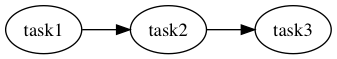
\includegraphics[width=0.5\textwidth]{./figures/workflow/tasks_flow_graph_trivialexample.png}
\end{center}
While in this case the flow chart is trivial, a real project will have a much more complicated structure that you can't remember.
See our \href{https://github.com/jdingel/DavisDingelMonrasMorales}{consumption segregation paper} for an example.

\subsection{All output is produced by tasks}

In reality, every number reported in your paper is produced by code.
Your workflow (and your replication package) therefore should produce every such number as a file in an \texttt{output} folder.
A summary statistic that appears in a sentence rather than in a table is still a code-produced number.
If you hardcode some number in your paper's \LaTeX\ file, I bet you'll forget to update it at least once (it's produced by code + human transcription and the latter is less reliable.)
I've certainly produced drafts where the same number takes different values in a paragraph and in a table because code produce the latter but not the former.

All output is produced by tasks.
Our task workflow produces the final paper.
See Patrick Ball at \href{https://www.youtube.com/watch?v=ZSunU9GQdcI&t=40m27s}{40:27}.

\section{Writing code} This section is for us to agree upon best practices in coding.
It's light at the moment.

\subsection{Language-free coding principles}

\subsubsection{Other people's principles}

\begin{itemize}
	\item See chapter 6, chapter 7, and appendix A of Gentzkow and Shapiro's \href{https://web.stanford.edu/~gentzkow/research/CodeAndData.pdf}{Code and Data for the Social Sciences: A Practitioner’s Guide}.
	\item QuantEcon's ``\href{https://julia.quantecon.org/getting_started_julia/introduction_to_types.html#A-Digression-on-Style-and-Naming}{A Digression on Style and Naming}''. Read their comments on the following:
	\begin{itemize}
	\item Code is read many more times than it is written
	\item Write code to be read in the future, not today
	\item Excess comments in code can make code harder to read
	\item Maintain the correspondence between the whiteboard math and the code
	\end{itemize}
\end{itemize}

\subsubsection{Do not hardcode values}

While I haven't fully embraced the \href{https://en.wikipedia.org/wiki/Functional_programming}{functional programming paradigm},
I do think that it is a mistake to use global variables or to hardcode values within functions.
See
Patrick Ball's \href{https://www.youtube.com/watch?v=ZSunU9GQdcI&t=36m43s}{argument}
and
page 28 of Gentzkow and Shapiro's \href{https://web.stanford.edu/~gentzkow/research/CodeAndData.pdf}{Code and Data}.

For example, sample selection decisions are arguments.
Constants do not belong inside functions.
Name them once, impose the value/criterion once, and then refer to that repeatedly within your function.
\href{http://yaml.org/}{YAML} is a good format for constants.

\subsection{Sharing code across machines}

We almost always want to run code on multiple machines.
Absolute file paths are problematic for shared code, because \texttt{/Users/jdingel/} is not a valid path for almost every computer on earth.
Here are two possible means of making shared code run on many machines:
\begin{enumerate}
	\item Set absolute file paths with conditional statements.
	\item Use only relative file paths.
\end{enumerate}

I strongly prefer the latter.

\subsubsection{Conditional absolute file paths}

Conditional absolute file paths exploit environmental variables to identify the machine and then set absolute file paths based on that.
For example, in Linux there is an environmental variable called \texttt{\$USER} at the shell command line.
Similarly, elements of Stata's c-class, such as \texttt{`c(pwd)'} and \texttt{`c(hostname)'}, can be used to identify a machine
and then run user-specific programs that set global variable to user-specific values.\footnote{
	Type \texttt{help creturn} in Stata for exhaustive documentation of the available arguments.
}
Here is a brief example in Stata.
\begin{lstlisting}[language=stata]
if "`c(os)'"=="Unix" & regexm("`c(hostname)'","midway")==1 {
	display "Running on RCC Midway server"
	global root "/project/xxx/xxxyyy/xyz_repo"
}
\end{lstlisting}

\subsubsection{Relative file paths}

Relative file paths work on any machine because they are relative.
In Jonathan's opinion, this is generally preferable.
It means that code can be cloned onto a new machine by any user and run immediately without having to write new user-specific code.
See \url{https://github.com/jdingel/DavisDingelMonrasMorales} for an example of a repository that only uses relative paths.

\href{https://help.github.com/articles/about-readmes/\#relative-links-and-image-paths-in-readme-files}{GitHub} agrees:
``Relative links are easier for users who clone your repository. Absolute links may not work in clones of your repository - we recommend using relative links to refer to other files within your repository.''

\subsubsection{Package management}

Package dependencies should be identified by \texttt{requirements.txt} (Python), \texttt{Manifest.toml} (Julia), and so forth.
Stata lacks a built-in package-dependency management tool.
These requirements should be committed to the repo so that anyone cloning the repo on a new machine has everything they need defined.
This is also \href{https://aeadataeditor.github.io/aea-de-guidance/preparing-for-data-deposit.html}{AEA journal policy}:
``packages/modules/etc. ... provide a setup program to install these (not manual instructions).''

\subsection{Limit lines to at most 100 characters}

Files should have lines no longer than 100 characters in length.
This is true both for code and \TeX.
The commands \texttt{diff} and \texttt{git diff} report lines that differ between files/commits.
Really long lines of code therefore can be a nightmare, since one may have to scroll quite far to spot a change.
This is really painful if a line is actually a full paragraph of text.
Writing each new sentence on a separate line makes it much easier to view changesets.

See \href{https://en.wikibooks.org/wiki/LaTeX/Collaborative_Writing_of_LaTeX_Documents\#Subversion_really_makes_the_difference}{Directives for using LaTeX with version control systems}
\begin{itemize}
\item Do not change line breaks without good reason.
\item Turn off automatic line wrapping of your LaTeX editor.
\item Start each new sentence in a new line.
\item Split long sentences into several lines so that each line has at most about 80 characters.
\item Verify that your code can be compiled flawlessly before committing your modifications to the repository.
\item Use diff to critically review your modifications before committing them to the repository.
\item Add a meaningful and descriptive comment when committing your modifications to the repository.
\end{itemize}

\section{Running code with Make} Projects consist of tasks that depend on each other.
If an upstream task changes, downstream tasks ought to be re-run using that new input.
This is easy to do by hand when your project has a small number of tasks.
This is hard to do when the tasks are computationally intensive and the input-output graph is complicated.
Thankfully, computer programmers addressed these difficulties long ago with a Unix utility called \href{https://en.wikipedia.org/wiki/Make_(software)}{Make}.
This is a popular form of the broader concept of \href{https://tradediversion.net/2019/11/06/why-your-research-project-needs-build-automation/}{build automation}.

Makefiles are machine-readable documentation that make your workflow reproducible.
They follow naturally from our task-based approach.
Downstream tasks depend on upstream tasks.
Using \texttt{make} requires you to specify those input-output relationship (dependencies).
When generated files are missing, or when files they depend on have changed, needed files are re-made using a sequence of commands you specify.
The commands are language-agnostic: if you can type it at the shell prompt,
\texttt{make} can execute it.

\subsection{Learn Make}

The \href{https://www.youtube.com/watch?v=_Ms1Z4xfqv4}{first fifteen minutes} of
\href{https://missing.csail.mit.edu/2020/metaprogramming/}{Lecture 8 in MIT's ``Missing Semester'' CS class}
are a great introduction to Make.
Start by watching that.

Here are four written introductions to \texttt{make}, listed in the order that I suggest reading them:
\begin{itemize}
\item Mike Bostock: \href{https://bost.ocks.org/mike/make/}{Why Use Make}
\item Karl Broman: \href{http://kbroman.org/minimal_make/}{minimal make}
\item Kieran Healy: \href{http://plain-text.co/pull-it-together.html}{Pull It Together} (The Plain Person's Guide to Plain Text Social Science)
\item Zachary M. Jones: \href{http://zmjones.com/make/}{GNU Make for Reproducible Data Analysis}
\end{itemize}

\subsection{Some simple examples of Makefiles}

The \texttt{Makefile} in the \texttt{logbook} folder is a simple example.
It compiles this PDF if \texttt{logbook.tex} or one of the elements of \texttt{\$(logbookentries)} is newer than \texttt{logbook.pdf}.

Here is an example of what a Makefile in an ``initialdata" task folder might do.
The following code is an excerpt from a Makefile that downloads Census data and produces a CSV by unzipping the downloaded file.
\begin{lstlisting}[language=make]
../output/mi_od_main_JT01_2010.csv: ../output/mi_od_main_JT01_2010.csv.gz
	gunzip -c $< > $@
../output/mi_od_main_JT01_2010.csv.gz: | ../output
	wget "https://lehd.ces.census.gov/data/lodes/LODES7/mi/od/$(@F)" -O ../output/$(@F)
../output:
	mkdir $@
\end{lstlisting}
The first rule concerns the target \texttt{../output/mi\_od\_main\_JT01\_2010.csv}.
The target lists a compressed file as its one pre-requisite.
If the target does not exist or if the target is older than (any of) the pre-requisite(s) listed after the colon,
then the recipe for that target is executed.
The recipe for this target is simple: use \texttt{gunzip} to decompress the pre-requisite and write it to the target.

Let's unpack that recipe in detail.
\href{https://linux.die.net/man/1/gunzip}{gunzip} takes a list of files on its command line and replaces each file whose name ends with .gz, -gz, .z, -z, \_z or .Z with an uncompressed file without the original extension.
\texttt{-c} is an option that writes output on standard output and keeps original files unchanged.
The somewhat cryptic \texttt{\$<} and \texttt{\$@} are \href{https://www.gnu.org/software/make/manual/html_node/Automatic-Variables.html}{automatic variables} in Make.
\texttt{\$<} is the first pre-requisite (\texttt{../output/mi\_od\_main\_JT01\_2010.csv.gz})
and
\texttt{\$@} is the target (\texttt{../output/mi\_od\_main\_JT01\_2010.csv}).
\texttt{>} redirects output to a file, overwriting the file.
(By the way, \texttt{>>} appends redirected output to the end of a file (rather than overwriting).)

The second rule defines the compressed file from Census as the target.
Its only pre-requisite is that the \texttt{../output} folder exist
(an ``order-only prerequisite'' indicated by the pipe \texttt{|}).
If \texttt{../output/} does not exist, the Makefile must provide a recipe to create it
(see lines 5-6).
The recipe for the compressed Census file is a \texttt{wget} command.
\texttt{wget} is a free utility for non-interactive download of files from the web
and \texttt{-O} is an option that concatenate all documents together and writes to the specified output file.
The automatic variable \texttt{\$(@F)} equals \texttt{mi\_od\_main\_JT01\_2010.csv.gz},
the file-within-directory part of the file name of the target.
It is used in specify the web address of the Census file.

If you type \texttt{make ../output/mi\_od\_main\_JT01\_2010.csv} at the command line, \texttt{make} will try to make the CSV target and see the CSV.GZ file as a pre-requisite.
If the pre-requisite has not been already downloaded, \texttt{make} will create the \texttt{../output} directory if needed,
then run the recipe to produce that CSV.GZ file (the \texttt{wget} command),
and then execute the recipe to produce the target.

After obtaining the initial data, we will use these data in (multiple) downstream tasks.
Here is an excerpt from the Makefile in a task called \texttt{LODES\_datapreparation}.
\begin{lstlisting}[language=make]
../output/lodes_DetroitUA_2010.dta: DetroitUA_tract.do programs.do ../input/mi_od_main_JT01_2010.csv | ../output
	$(STATA) $<
../input/mi_od_main_JT01_2010.csv: ../../LODES_downloaddata/output/mi_od_main_JT01_2010.csv | ../input
	ln -s $< $@
../../%:
	$(MAKE) -C $(subst output/,code/,$(dir $@)) ../output/$(notdir $@)
\end{lstlisting}
This target \texttt{../output/lodes\_DetroitUA\_2010.dta} has four pre-requisites:
\texttt{DetroitUA\_tract.do}, \texttt{programs.do}, the CSV file that we described downloading above, and the \texttt{output} folder.
The recipe for this target is to run the Stata script \texttt{DetroitUA\_tract.do} (referenced by \texttt{\$<}).
\$(STATA)\$ is an alias for how we invoke Stata
(modified to return a proper exit status and work with SLURM, ignore those details for now).
In lines 3-4, \texttt{ln -s} creates a symbolic link called \texttt{../input/mi\_od\_main\_JT01\_2010.csv} that points to the upstream file
\texttt{../../LODES\_downloaddata/output/mi\_od\_main\_JT01\_2010.csv}.
The final two lines define a generic recipe for producing upstream content.
The \texttt{\%} is a wildcard, so this recipe will be used for \textit{any} target whose path starts with \texttt{../../}.
\texttt{../../LODES\_downloaddata/output/mi\_od\_main\_JT01\_2010.csv} is an example of such a target.
If this file isn't already available,
the recipe runs \texttt{make} in the upstream folder
\texttt{../../LODES\_downloaddata/code}.
Notice that it invokes a different Makefile (the one assumed to be in the \texttt{LODES\_downloaddata} task)
in order to produce the target.

\subsection{Notes on writing Makefiles}

An important reminder: Each line in the recipe must start with a tab.
See \href{https://www.gnu.org/software/make/manual/html_node/Recipe-Syntax.html}{Recipe Syntax}.

A few notes on Makefile style.
\begin{itemize}
\item
When you run \texttt{make} without specifying a target,
its \href{https://www.gnu.org/software/make/manual/html_node/How-Make-Works.html#How-Make-Works}{default goal}
is to build the first target listed in the file.
Convention is to define \texttt{all} as the first target of the Makefile and list all desired targets as pre-requisites of \texttt{all}.
\item It is helpful to define \href{https://www.gnu.org/software/make/manual/html_node/Variables-Simplify.html#Variables-Simplify}{variables} containing long lists of files, such as \texttt{INPUTS= file1 file2 file3}
so that you can summarize dependencies simply by writing \texttt{\$(INPUTS)}
and define targets simply by writing \texttt{all: \$(INPUTS) \$(OUTPUTS)}.
However, it is only sensible to write a target-dependency relationship as
\texttt{\$(OUTPUTS): \$(INPUTS)}
if there is one recipe that produces all those outputs jointly.
\item Writing separate recipes for separate targets is advantageous because Make will return more informative errors by telling you which recipe failed.
\item \href{https://www.gnu.org/software/make/manual/html_node/Automatic-Variables.html}{Automatic variables} take values computed when the rule is executed based on the target and pre-requisites of the rule.
Commonly used automatic variables include
the file name of the target of the rule \texttt{\$@},
the name of the first pre-requisite \texttt{\$<},
and
the file-within-directory part of the file name of the target \texttt{\$(@F)}.
\item In addition to normal prerequisites, it might be helpful to define \href{https://www.gnu.org/software/make/manual/html_node/Prerequisite-Types.html}{order-only prerequisites}.
Order-only prerequisites must exist in order for the target to be produced, but the target does not need to be newer than the order-only prerequisites.
An example of prerequisites that should be regarded as order-only is folders, since ``the timestamps on directories change whenever a file is added, removed, or renamed, we certainly don’t want to rebuild all the targets whenever the directory’s timestamp changes'' (\href{https://www.gnu.org/software/make/manual/html_node/Prerequisite-Types.html}{GNU}).
Order-only prerequisites are defined by listing them after the pipe symbol: \texttt{output: normal prerequisites | order-only prerequisites}.
\item Make provides several built-in \href{https://www.gnu.org/software/make/manual/html_node/Functions.html\#Functions}{functions for transforming text}.
Commonly used functions include \texttt{foreach} for performing text substitution by looping
and \texttt{addprefix} for prepending prefix in front of individual names.
\item In addition to executing recipes in the shell, you can define Make variables using shell commands by invoking Make's \texttt{shell} command.
The simplest example would \texttt{\$(shell echo \{1..10\})}, which would return the integers from 1 to 10 via Bash's \href{https://www.shell-tips.com/bash/seq-brace-expansion/}{brace expansion}.
\end{itemize}

\textbf{Grouped targets}.
Historically, Make (like most of neoclassical economics) has assumed
``\href{https://doi.org/10.2307/2525367}{no joint production}''.
If two targets are produced by the same recipe, Make assumes it needs to run the recipe twice.
Consider this trivial shell script (\texttt{joint\_producer.sh})
\begin{lstlisting}[language=bash]
echo 'done' > output1.txt
echo 'done' > output2.txt
\end{lstlisting}
accompanied by this trivial Makefile:
\begin{lstlisting}[language=make]
all: output1.txt output2.txt
output1.txt output2.txt:
	bash joint_producer.sh
\end{lstlisting}
Running the script once will produce both outputs.
But what does Make think you need to do? Run it twice.
In practice, after the first run, Make will see that the second target has been produced.
But if you run Make with parallel threads, it will run the script twice simultaneously.
\begin{lstlisting}[language=bash]
jdingel$ make -n
bash joint_producer.sh
bash joint_producer.sh
jdingel$ make
bash joint_producer.sh
jdingel$ rm output?.txt
jdingel$ make -j 2
bash joint_producer.sh
bash joint_producer.sh
\end{lstlisting}
Make 4.3 (\href{https://lwn.net/Articles/810071/}{January 2020 release}) introduced
``\href{https://www.gnu.org/software/make/manual/html_node/Multiple-Targets.html}{grouped targets}'',
thereby allowing joint production.
Make 4.3 would not make the mistake of submitting two copies of the same job when running parallel threads if you define the targets as grouped by \texttt{output1.txt output2.txt \&:},
where the ampersand indicates grouped targets.
I have typically refrained from using grouped targets because one cannot assume Make 4.3 will be available on most boxes (e.g., Midway2 is running GNU Make 3.82).

A note on running Makefiles in a cluster computing environment that has a job scheduler:
\begin{itemize}
	\item A problem with batch jobs is that the shell sees the submission command as completed upon job submission any output files are produced.
	Failing to see the output, Make will repeatedly submit the job.
	\item You need the job submission command to not exit back to the shell until the job completes, so that the target will be produced before Make evaluates that recipe's success or failure.
	\item With PBSPro's \texttt{qsub} at Census RDC, use \texttt{qsub -W block=true}.
	\item With SLURM's \texttt{sbatch} at Chicago Midway, use \texttt{sbatch -W}.
	\item Read \url{http://wresch.github.io/2012/11/01/qsub-submit-jobs-from-makefile.html} for more discussion of \texttt{qsub} and the \texttt{sbatch} \href{https://slurm.schedmd.com/sbatch.html}{manual} for discussion of \texttt{-W} or \texttt{--wait}.
	\item I am not sure about the best practice for the Torque scheduler.
\end{itemize}


The following options are often relevant:
\begin{itemize}
	\item \texttt{-n}: Prints the recipes that would be executed without executing them. Great to preview what jobs you're going to launch by running Make.
	\item \texttt{-j}: this option allows parallelization of jobs, i.e., contemporaneous execution of several recepies.
	Normally, make executes one recipe at a time, but \texttt{-j} enables simultaneous execution.
	\texttt{-j} is followed by an integer specifying the number of parallel processes.
	The default number of jobs run is 1 (serial processing).
	\item \texttt{--debug}: this option is useful to know how make analyzes your dependency graph. This option provides the most detailed information available other than running a debugger.
	We make use of 2 suboptions of \texttt{--debug}: ``basic'' and ``verbose''.
	When the ``basic'' suboption is used, make will print each target that is found out-of-date and the status of the update action.
	``verbose'' replicates the ``basic'' suboption and includes additional information about files that were parsed, prerequisites that did not need to be rebuilt, etc.
\end{itemize}

\section{Tracking code with Git} This section introduces the idea of version control and applies it to a single-machine user.
(This is sufficient for applying version control to confidential-data settings where you only work on one server.)
A later section in the \textbf{Collaboration} block addresses using version control when sharing across machines.

\subsection{Introduction to version control}

Version control is the management of changes to code and documents.
It should be applied to all textual content in a research project.
Version control tools allow us to
\begin{itemize}
	\item Keep a complete history of our project without any additional effort or files
	\item Hit ``undo'' (at arbitrarily large scale) at will
	\item Collaboration: Edit code simultaneously without creating disastrous conflicts
	\item Collaboration: Easily track coauthors' contributions and changes
\end{itemize}
All real programmers use version control. The dominant version control software is Git.

To understand version control, please read the following short introductions:
\begin{itemize}
	\item Gentzkow \& Shapiro - ``\href{https://web.stanford.edu/~gentzkow/research/CodeAndData.pdf}{Chapter 3: Version Control}''
	\item Michael Stepner - ``\href{https://michaelstepner.com/blog/git-vs-dropbox}{git vs. Dropbox from a researcher's perspective}''
\end{itemize}

\subsection{Which files should be kept in version control?}

Version control is appropriate for any plaintext file.
Binaries (like PDFs) are less suitable, since you can't examine their contents.

Obviously all code should be in version control. What about writing?
\begin{itemize}
	\item \LaTeX\ is perfect; it's plaintext.
	\item LyX is suitable for version control, because \texttt{.lyx} files are plaintext.
	\item Jonathan prefers to err on the side of documenting and committing too much. There's little downside.
\end{itemize}

A file called \texttt{.gitignore} identifies paths that should not be tracked by Git.
\begin{itemize}
\item
We don't commit data.
I therefore typically put \texttt{tasks/*/output} in \texttt{.gitignore} so that the repository doesn't track output files.
\item
Git sees symbolic links as their targets.
I therefore put \texttt{tasks/*/input} in \texttt{.gitignore} so that the repository doesn't track data files.
\item
To produce logbook content (and the paper), you may want to commit tables and figures from these output folders.
To do so, you can always type, for example, \texttt{git add table1.tex -f}, where the \texttt{-f} force option causes the file to be tracked despite the gitignore rule.
\end{itemize}

\subsection{Version control in a single-machine environment}

To productively use git in a single-machine environment, you only need to know a half-dozen commands.
\begin{itemize}
\item \texttt{git init} initializes a repository in the current working directory
\item \texttt{git status} tells you what files have been modified since you last committed
\item \texttt{git diff} shows you those modifications (and can also show you the modifications between any two commits)
\item \texttt{git add} stages a file
\item \texttt{git commit} commits a set of changes
\item \texttt{git log} lists the history of commits
\end{itemize}
See ``\href{https://git-scm.com/book/en/v1/Git-Basics}{Git Basics}'' on these.

A couple more resources:
\begin{itemize}
\item For command-line Git, see Atlassian's \href{https://www.atlassian.com/git/tutorials/atlassian-git-cheatsheet}{Git cheatsheet}.
\item You may also want to glance at Jess Johnson - \href{http://www.grokcode.com/717/how-to-use-source-control-effectively/}{How To Use Source Control Effectively}.
\item If your University subscribes to Lynda, they offer \href{https://www.lynda.com/search?q=git}{a number of Git courses} (with which I have no experience).
\end{itemize}




Some notes on command-line Git by Ningyin Xu, a former RA, follow.

\subsubsection{Setting up a repository}

If you want to create a brand-new repo, you'll use the \texttt{git init} command.
\begin{lstlisting}[language=bash]
cd /path/to/your/existing/project
git init
\end{lstlisting}

\subsubsection{Saving changes to the repository}
Now that we have a repository, we can edit its contents and then commit changes to it.
The basic commands are:
\begin{lstlisting}[language=bash]
cd /path/to/repo
# make some changes to a file named "test.txt"
git add test.txt
git commit -m "edited test.txt"
\end{lstlisting}
This example introduced two additional git commands: \texttt{add} and \texttt{commit}.
The \texttt{git add} command adds a change in the working directory to the staging area.
It tells Git that you want to include updates to a particular file in the next commit.
However, \texttt{git add} doesn't really affect the repository in any significant way — changes are not actually recorded until you run \texttt{git commit}.
The \texttt{git commit} command commits the staged snapshot to the project history.
Committed snapshots can be thought of as ``saved'' versions of a project, Git will never change them unless you explicity ask it to.
In conjunction with these commands, you'll also need \texttt{git status} to view the state of the working directory and the staging area.
In general cases, you could do ``git status'' before ``git add'', and Git will tell you what files you have made changes and how you could deal with them.

Another common use case for \texttt{git add} is the \texttt{--all} option.
Executing \texttt{git add --all} will take any changed and untracked files in the repo and
add them to the repo and update the repo's working tree.
This may include hidden files.
You should list files that you do not want to be part of the repository in the file called \texttt{.gitignore} (\href{https://git-scm.com/docs/gitignore}{documentation}).


\subsubsection{Undoing changes}
The \texttt{git checkout} command is mostly used for its three functions:
checking out files, checking out commits, and checking out branches.
Checking out a commit makes the entire working directory match that commit.
This can be used to view an old state of your project without altering your current state in any way.
Checking out a file lets you see an old version of that particular file, leaving the rest of your working directory untouched.
Checking out branches will be discussed in the \textbf{Collaboration} section.
\\
\begin{lstlisting}[language=bash]
git checkout <commit> <file>
# Check out a previous version of a file. This turns the <file> that resides
# in the working directory into an exact copy of the one from <commit> and
# adds it to the staging area.

git checkout <commit>
# Update all files in the working directory to match the specified commit.
# But this is a read-only operation, the ``current'' state of your project
# remains untouched in the master branch.

git checkout master
# This lets you to get back to the "current" state (under the condition you
# don't have more than one branches).
\end{lstlisting}

In some case, you might want to undo your last commit.
To do that, use \texttt{git reset --soft HEAD\texttt{$\sim$}1}.
This command will remove the last commit from the current branch and keep previously commited files in the staged area.
For a more detailed description, see \href{https://www.atlassian.com/git/tutorials/undoing-changes/git-reset}{Atlassian guide}.


\section{Sharing code via Git} 
Git's true powers lie in the fact it is a \textit{distributed} version-control system for tracking changes.
Every Git directory on every computer is a full-fledged repository with complete history and full version-tracking abilities, independent of network access or a central server.

In projects involving multiple machines,
collaborating on a repository involves distinguishing between the ``local'' and ``remote'' repos.
It involves (at least) three new git commands: \texttt{git clone}, \texttt{git pull}, and \texttt{git push}.

Take a look at Figures 3 and 4 in
Blischak JD, Davenport ER, Wilson G (2016)
``\href{http://journals.plos.org/ploscompbiol/article?id=10.1371/journal.pcbi.1004668}{A Quick Introduction to Version Control with Git and GitHub}.'' \textit{PLoS Comput Biol} 12(1): e1004668.

Try Roger Dudler - \href{http://rogerdudler.github.io/git-guide/}{git - the simple guide}.
After reading the material below, you might also circle back to read
the ``\href{https://github.com/OpenSourceMacro/BootCamp2017/blob/master/Tutorials/git_tutorial.pdf}{Git tutorial}''
from UChicago's Open Source Macroeconomics Laboratory.

\subsection{Online hosting services and a GUI client}

Don't confuse Git and GitHub.
Git is free, open-source software.
\href{http://www.github.com}{GitHub}, \href{https://bitbucket.org/}{BitBucket}, and GitLab are
online repository hosting services.
They also provide a number of user-friendly GUI tools for code review and commenting that complement Git.

While you can run Git from the command line,
you might find it a little easier to have a GUI as you learn Git.
I recommend using \href{https://www.sourcetreeapp.com/}{SourceTree},
a free Git GUI for OS X, although it's the only Git GUI I've used.\footnote{
	Some of my coauthors have had poor experiences using SourceTree on their Windows machines.
}
SourceTree is by Atlassian, the folks also behind BitBucket.
You can \href{https://confluence.atlassian.com/get-started-with-sourcetree/work-using-git-847359053.html}{use the app to} pull, commit, push, diff, etc.
If you're on Windows, perhaps try \href{https://www.gitkraken.com/}{GitKraken}.

\subsection{Clone the remote repo}

If you want to create a local development clone of an existing repo,
give the \texttt{git clone} command a repository URL to create a copy of the remote repo.
Then the content is on your machine as a local repo.
For example, to clone the (public) remote repo ``lights\_to\_cities''
\begin{lstlisting}[language=bash]
cd path/you/want/to/put/the/repo
git clone https://github.com/jdingel/lights_to_cities.git
\end{lstlisting}

Here's another example, this time cloning a private repository hosted by BitBucket.
Log in to Bitbucket.org and go to the \texttt{beacensus} repository page:
\url{https://bitbucket.org/jdingel/beacensus}.
On the repository page, click the

\includegraphics[width=.025\textwidth]{./figures/workflow/BitBucket_screeshot_cloneinsourcetree2.png}
button and you'll be prompted to clone the repository to your own machine using the SourceTree application.
\begin{center}
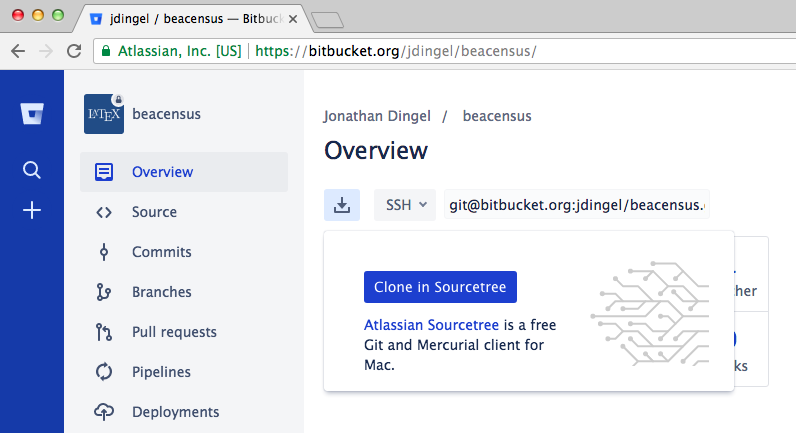
\includegraphics[width=.8\textwidth]{./figures/workflow/BitBucket_screeshot_cloneinsourcetree1.png}
\end{center}
Name the folder on your machine, and a copy of all the files in the remote repository will be cloned to your local repository.

It's also possible to clone remote repositories to which you have access simply by opening the SourceTree app and following \href{https://confluence.atlassian.com/get-started-with-sourcetree/clone-a-remote-repository-847359098.html}{these instructions}.

\subsubsection{Pull and push}

Two commands, \textbf{git pull} and \textbf{git push},
allow us to sync the local repo and remote repo.
You ``pull'' commits from the remote repo down to your local repo;
you ``push'' commits from your local repo to the cloud.

You must pull before you push.
You can pull after you commit, but if you commit and there are already new commits in the remote repo, you have to pull those commits and merge them with yours before you're allowed to push your commit to the remote repo.\footnote{
	Git Basics \href{https://git-scm.com/book/en/v2/Git-Basics-Working-with-Remotes\#_pushing_remotes}{2.5} on \texttt{git push}: ``This command works only if you cloned from a server to which you have write access and if nobody has pushed in the meantime. If you and someone else clone at the same time and they push upstream and then you push upstream, your push will rightly be rejected. You'll have to fetch their work first and incorporate it into yours before you'll be allowed to push.''
}
It's best to pull before you commit, just to reduce the number of ``merge'' commits that appear in the project history.
But if you're working on the same file as a collaborator, merges are unavoidable.
Git isn't Dropbox: if you ignore a project for a couple weeks, nothing will sync automatically.
But there's no reason to pull regularly if you're not looking at a project.
Pull when you sit down to resume work.

Relative to the single-machine process of doing a chunk of work and committing it,
the collaborative process involves only one extra step:
push after you commit.
\begin{lstlisting}[language=bash]
cd /path/to/repo
git pull
# make some changes to a file named "test.txt"
git add test.txt
git commit -m "edited test.txt"
git push
\end{lstlisting}


\subsubsection{Branching and merging}
A branch is series of commits that can be distinguished from another collection of commits.
Branches allow you to make commits without immediately having that code be imposed on the master project.
The merit of branching is most obvious when you're doing web development in which your service is always ``live''.
If the ``master'' branch is your live website, you don't want version 0.1 of a new feature to immediately go live.
In that case, the master branch must be immaculate, and branches are where development happens.
Once new features (or rewrites of old features) are tested and proven, they're merged into the master branch.

Research doesn't quite follow this model.
It's unlikely that there's a ``live'' version.
On the other hand, we often rewrite code when something is slow or inefficient.
For large chunks of work (or for rewrites that should deliver identical output), it makes sense to work on your own branch so that others' downstream work isn't altered until you're ready to merge into the master branch.
We create a new branch whenever we create a new task or substantially rewrite an old task.
See Section~\ref{code_review_process} for more about the role of branching within our code writing and reviewing processes.

The \texttt{git branch} command lets you create, list, rename, and delete branches.
It is tightly integrated with the \texttt{git checkout} and \texttt{git merge} commands.
\begin{lstlisting}[language=bash]
git branch
# List all of the branches in your repository.

git branch <branch>
# Create a new branch called <branch>. This does not check out the new branch.

git branch -d <branch>
# Delete the specified branch. This is a ``safe'' operation in that Git prevents
# you from deleting the branch if it has unmerged changes.

git branch -D <branch>
# Force delete the specified branch, even if it has unmerged changes. This is
# the command to use if you want to permanently throw away all of the commits
# associated with a particular line of development.

git branch -m <branch>
# Rename the current branch to <branch>.

git checkout <existing-branch>
# Check out the specified branch, which should have already been created with
# git branch. This makes <existing-branch> the current branch, and updates the
# working directory to match.

git checkout -b <new-branch>
# Create and check out <new-branch>. The -b option is a convenience flag that
# tells Git to run git branch <new-branch> before running git checkout
# <new-branch>. git checkout -b <new-branch> <existing-branch>

git merge <branch>
# Merge the specified branch into the current branch. Git will determine the
# merge algorithm automatically (discussed below).

git merge --no-ff <branch>
# Merge the specified branch into the current branch, but always generate a
# merge commit (even if it was a fast-forward merge).
\end{lstlisting}

In some cases, you might forget to pull the latest commit before making a new one.
As a result, you might be unable to push your commit due to a \href{https://happygitwithr.com/push-rejected.html}{conflict} with the latest commit on a repository.
To find a solution, read \href{https://happygitwithr.com/pull-tricky.html}{Chapter 28 Pull, but you have local work}.

\section{Sharing results via the logbook} 
This logbook is where we document the research project.
It can present preliminary results, sketch empirical specifications, etc.
There are separate chapters for research infrastructure, call notes, and research results.
These categories are easy to revise -- individual logbook entries should be modular pieces suitable for re-ordering.
Within chapters, entries are usually ordered chronologically. Entries are identified by date and author.
At their best, logbook entries presenting results can be directly pasted into the first draft of the paper.

\subsection{Committing logbook entries}

To add an entry this logbook:
\begin{enumerate}
	\item Write the logbook entry as a \TeX\ file. The \TeX\ file will be embedded within the logbook \TeX\ file, so do not include any \LaTeX\ preamble.
	\item Insert the entry into the logbook by editing \texttt{logbook.tex}.
	The logbook entry (section) title should include an informative title, the date, and author.
	Follow it by \texttt{\textbackslash input\{\}} with the filename.
	All other content is in the entries' individual \TeX\ files.
\end{enumerate}

What not to commit
\begin{itemize}
	\item Please do not commit the logbook PDF to the repository.
	Doing so often creates merge conflicts when users preview their own logbook entries by compiling the logbook PDF locally.
	Similarly, do not commit the paper PDF to the repository.
	\item Do not commit the \texttt{logbook.aux}, \texttt{logbook.log}, nor \texttt{logbook.out} files generated by your \LaTeX compiler.
	Either add these to your \texttt{.gitignore} file or have your Makefile delete these after succesful compilation of the PDF.
\end{itemize}


\section{Unix/Linux shell commands} \label{entry:unixshelltips}

This section documents basic Unix/Linux shell commands and then some clever combinations for tasks we often encounter during research.
At the command line, type \texttt{man <<command>>} to get the \href{https://en.wikipedia.org/wiki/Man_page}{manual page} for \texttt{<<comand>>}.

\subsection{Mac OS X is Unix and POSIX-compliant, not GNU/Linux}

Mac OS X is based on the Darwin operating system, which is based on BSD.
It \href{https://www.opengroup.org/openbrand/register/apple.htm}{counts as UNIX} and is POSIX-compliant.
But it is not GNU/Linux.
You will therefore run into annoying differences when trying to use some utilities, mostly when you see a solution on StackExchange that works on GNU/Linux but doesn't work on Mac OS X.
Here's a short list:
\begin{itemize}
\item \texttt{tree} not available in OS X by default, please run \texttt{brew install tree} to install it via Homebrew.
\item \texttt{cut} lacks the complement option in OS X
\item \texttt{wc} lacks the \texttt{-L, --max-line-length} option available in \href{https://linux.die.net/man/1/wc}{Linux}.
\item Unfortunately, \texttt{sed} differs considerably between GNU and OS X.
\begin{itemize}
	\item The \texttt{-i} option syntax \href{https://stackoverflow.com/questions/2320564/i-need-my-sed-i-command-for-in-place-editing-to-work-with-both-gnu-sed-and-bsd}{differs} between GNU and OS X
	\item GNU sed \href{https://unix.stackexchange.com/questions/13711/differences-between-sed-on-mac-osx-and-other-standard-sed}{supports} \texttt{\textbackslash|}, \texttt{\textbackslash+}, and \texttt{\textbackslash?} in regular expressions but OS X (and POSIX) don't.
	\item Other warnings (\href{https://unix.stackexchange.com/a/131940}{1},\href{https://stackoverflow.com/questions/1227174/sed-on-os-x-cant-seem-to-use-in-regexps}{2}), like the \texttt{-e} flag will give you extended regular expressions in OS X but isn't really compatible with Linux.
\end{itemize}


\end{itemize}


\subsection{Navigating the file system}

\begin{itemize}
	\item \texttt{pwd}: identify the ``present working directory''
	\item \texttt{cd}: ``change directory'' to the named destination (e.g., \texttt{cd <<destination>>})
	\item \texttt{ls -lht}: lists the current directory's contents. The \texttt{-lht} options list the files in detail, with human-readable file sizes, ordered by time last modified.
	\item \href{https://en.wikipedia.org/wiki/Command-line_completion}{tab completion}:
	You do not have to type a complete filename. Starting typing the file name and hit the \texttt{tab} key.
	Commands with long or difficult to spell filenames can be entered by typing the first few characters and pressing a completion key, which completes the command or filename.
	\item To recall a command from your \href{https://www.howtogeek.com/howto/44997/how-to-use-bash-history-to-improve-your-command-line-productivity/}{history}, type \texttt{ctrl-R} to search and type a fragment of the command
	\item hashtag comments: comments in the shell are set off by \texttt{\#}. add a comment to your command to tag it for easier retrieval via search in the future
	\item copy files using \texttt{cp}, move files using \texttt{mv}
	\item copy files across different servers using \href{https://kb.iu.edu/d/agye}{scp}
\end{itemize}

\subsection{Navigating text}

\begin{itemize}
	\item \texttt{ctrl-A} jumps to beginning of line
	\item \texttt{ctrl-E} jumps to end of line
	\item \texttt{ctrl-K} kills content (cuts) from cursor to end of line
	\item \texttt{ctrl-U} kills content (cuts) from cursor to beginning of line
\end{itemize}

\subsection{Piping and writing to file}
A \href{https://en.wikipedia.org/wiki/Pipeline_(Unix)}{pipeline} is a sequence of processes chained together by their standard streams, so that the output of each process feeds directly as input to the next one.
Pipe using \texttt{|}.

To write output to a file, use \texttt{>}.
This overwrites the file if it already exists.
Use \texttt{>>} to append to an existing file.


\begin{itemize}
	\item parse a directory listing using \texttt{grep}: the command
	\begin{verbatim}ls -l | grep 'key'\end{verbatim}
	will output the directory listing and select only the lines containing the phrase ``key''
	\item write hello world to a file:
	\begin{verbatim}echo 'hello world' > file.txt\end{verbatim}
	\item look for missing files in a numbered sequence:
		  \begin{verbatim}
		  ls ../output/isoindices_{1..500}.dta > /dev/null
		  \end{verbatim}
		  This returns only the files that are not found in that \href{http://www.thelinuxrain.com/articles/building-sequences-of-numbers-on-the-command-line}{sequence}.
		  (the null device is a device file that discards all data written to it but reports that the write operation succeeded)
\end{itemize}

\subsection{Text processing}

\begin{itemize}
	\item \texttt{cat}: Reads files sequentially, writing them to standard output. The name is derived from its function to concatenate files. At the command line, think of this as ``print the file''.
	\item \texttt{head -n <filename>} outputs the first \texttt{n} lines of the file. the default is ten lines
	\item \texttt{tail -n <filename>} outputs the last \texttt{n} lines of the file. the default is ten lines
	\item \texttt{grep}: returns all lines of a file matching a specified expression (use \texttt{-v} option to return all lines not containing the expression)
	\begin{itemize}
		\item how to \href{https://stackoverflow.com/questions/29465612/how-to-detect-invalid-utf8-unicode-binary-in-a-text-file}{detect invalid utf8} unicode/binary in a text file: \texttt{grep -axv '.*' file.txt}
	\end{itemize}
	\item \texttt{sed}: stream editor with many functions; I mostly use it to substitute one expression for another
	\item \texttt{tr}: change or delete characters. It is useful for changing filenames (e.g. deleting whitespace).
	\item \texttt{awk}: find and replace text, print columns, a number of other text editing functions
	\begin{itemize}
		\item \href{https://developer.ibm.com/tutorials/l-awk1/}{An intro to the great language with the strange name} (Daniel Robbins, 1 Dec 2000)
		\item \href{https://gregable.com/2010/09/why-you-should-know-just-little-awk.html}{Why you should learn just a little Awk} (Greg Grothaus, 29 Sep 2010)
	\end{itemize}
	\item \texttt{paste}: horizontally concatenate files with equal number of lines
\end{itemize}

Combine these well and you get something like
``\href{https://adamdrake.com/command-line-tools-can-be-235x-faster-than-your-hadoop-cluster.html}{Command-line Tools can be 235x Faster than your Hadoop Cluster}''.

\subsection{Emacs}

Most often, you'll be an environment where you get to choose your own text editor.
However, in some (i.e., confidential) computing environments, you will not be free to install arbitrary software.
Emacs will typically be installed everywhere, so it it worth knowing some basic info.

\href{https://en.wikipedia.org/wiki/Emacs}{Emacs} is a family of text editors, dating to the 1970s, that is ``the extensible, customizable, self-documenting, real-time display editor.''
But there's a learning curve.
Even \href{https://www.gnu.org/software/emacs/tour/}{the introductions} can be overwhelming.

With regard to Emacs \href{https://www.emacswiki.org/emacs/EmacsKeyNotation}{key notation},
\texttt{C} means the ``control'' key and \texttt{M} means the alt/option key.

\begin{itemize}
	\item Quitting/exiting: \texttt{C-x C-c}
	\item Saving: \texttt{C-x C-s}
	\item \href{https://www.emacswiki.org/emacs/CopyAndPaste}{Copy and paste}:
	The selected region is where your cursor is relative to where you set a mark.
	Set a mark with C-space.
	Then move your cursor to end of region and hit C-w to cut (kill) or M-w to copy.
	Paste using C-y (yank).

\end{itemize}

\subsection{Multiple ``windows''}

\href{https://www.gnu.org/software/screen/manual/}{Screen} is ``a full-screen window manager that multiplexes a physical terminal between several processes, typically interactive shells.''
Consider using this if you want, e.g., to run Stata interactively in the bottom half of your screen while working on your do file in a text editor in the top half.

\subsection{Data compression}
In macOS, using the Finder to compress files produces hidden files that are useless to non-Mac users.%
\footnote{For details, see \url{https://perishablepress.com/remove-macosx-ds-store-zip-files-mac/}.}
In addition, the Finder does not use the ZIP64 extension to compress files what may make large ZIP files unreadable by other machines.
To avoid these issues, compress data by using the Terminal command line instead of the Finder.
The following Unix utilities are available to compress or decompress data:
\begin{itemize}
	\item \texttt{tar} for tar archive format
	\item \texttt{zip} for zip archive format.
	\item \texttt{gzip} for gz archive format.
\end{itemize}

When compresing files, it might be also useful to store the names of saved file without storing the directories.
In zip utility, it can be done using option \texttt{-j} to junk the paths.


\subsection{SLURM (Simple Linux Utility for Resource Management)}

Read the \href{https://rcc.uchicago.edu/docs/using-midway/index.html#batch-jobs}{RCC introduction} and then head over to the \href{https://slurm.schedmd.com/overview.html}{official documentation}.
To understand how the RCC compute ecosystem and get futher information on RCC usage, read \href{https://github.com/rcc-uchicago/SLURM_Workshop_2020/blob/main/Slides/Running_Jobs_at_RCC_fall.pdf}{slides from UChicago Slurm workshop.}
This \href{https://slurm.schedmd.com/pdfs/summary.pdf}{two-page PDF} lists almost all the relevant commands you might need.

\begin{itemize}
	\item \texttt{sbatch}: this command submits jobs (\texttt{.sbatch} scripts) to the job scheduler on the cluster
	\begin{itemize}
		\item Instead of writing a separate sbatch file for each script you might want to run using SLURM, you can pass the particular script/filename as an argument using the \texttt{--export} option.
		\item It is possible to set job dependencies in Slurm:
		Slurm will not start a job until the specified dependecies are satified.
		To set job dependencies, specify the dependency type and job ID in \texttt{--dependency} option.
	\end{itemize}
	\item \texttt{sinteractive}: start an interactive session on the server
	\item \texttt{squeue --user=jdingel}: list running and queued jobs for the relevant users
	\item My preferred \texttt{squeue} command is the following:
	\begin{lstlisting}[language=bash]
	squeue --user=jdingel  --format="%.17i %.13P %.20j %.8u %.8T %.9M %.9l %.6D %R" #jdjobs
	\end{lstlisting}
	This provides a good bit more information about each job.
	\item \texttt{rcchelp sinfo}: produce a summary of the partitions on Midway
	\item How to only see really costly jobs:
	\begin{lstlisting}[language=bash]
	rcchelp usage --byjob | grep '[0-9][0-9][0-9]\.[0-9][0-9][[:blank:]]|'
	\end{lstlisting}
	Without options, \texttt{rcchelp usage --byjob} provides a complete history of job submissions.
	Piping it to grep to select only lines containing a number in the form \#\#\#.\#\# returns only jobs that used at least 100 service units.
\end{itemize}

\subsection{Jumping between MacOS GUI and Terminal}

A few tips if you're using Terminal on your Mac but not a 100\% command-line ninja:
\begin{itemize}
	\item You can drag the path of a Mac folder into Terminal (or Stata) by dragging the folder icon at the top of its Finder window into the Terminal prompt (\href{https://twitter.com/lukestein/status/1179792864630296578}{via Luke Stein})
	\item Typing \texttt{`open . `} in any directory in the Terminal will open that folder in the Finder (\href{https://twitter.com/FlorianOswald/status/1179779138892292096}{via Florian Oswald})
\end{itemize}

\subsection{Other resources}

\begin{itemize}
	\item \url{https://unix.stackexchange.com/questions/6/what-are-your-favorite-command-line-features-or-tricks}
	\item MIT's \href{https://hacker-tools.github.io/}{Hacker Tools} course
	\item UChicago \href{https://rcc.uchicago.edu/support-and-services/workshops-and-training}{RCC Workshops and Training}
\end{itemize}

\section{Aesthetics and visualization} These are Jonathan's standards and he's willing to argue for them.

\begin{itemize}
	\item Generally, follow Edward Tufte's \href{https://www.edwardtufte.com/tufte/books_vdqi}{\textit{Visual Display of Quantitative Information}}.
	Mostly important, maximize the \href{https://www.coursera.org/learn/python-plotting/lecture/qFnP9/graphical-heuristics-data-ink-ratio-edward-tufte}{data-ink ratio}.
	\item At minimum, let's adhere to Schwabish ``\href{https://www.aeaweb.org/articles?id=10.1257/jep.28.1.209}{An Economist's Guide to Visualizing Data}'' (\textit{JEP} 2014)
	\item Never make a graphic with fewer than a dozen data points. A dozen data points belong in a table.
	\item Please impose \texttt{graphregion(color(white))} on every \texttt{twoway} plot created in Stata.
\end{itemize}

\section{Manuscript preparation} Before distributing a draft, use automated tools to validate the text.
Within \texttt{paper/reviewing}, there is a Makefile that
\begin{itemize}
	\item reports repeated words to avoid ``the the'' errors
	\item changes references to be ``tight'': \texttt{Table$\scriptstyle\sim$\textbackslash{}ref} rather than \texttt{Table \textbackslash{}ref}
	\item prints hard-coded numbers for verification or replacement
	\item runs ChkTeX to check \LaTeX semantics
	\item runs TeXtidote to check grammar and spelling
\end{itemize}

\begin{itemize}
\item
If you haven't installed \href{https://ctan.org/pkg/chktex?lang=en}{ChkTeX}, Macintosh installation instrutions are available at \url{http://www2.hawaii.edu/~ramonf/ChkTeXonMacOSX/index.html}.
\item
TeXtidote is available from \url{https://github.com/sylvainhalle/textidote}.
To install on Mac OS X, install the \href{https://www.oracle.com/technetwork/java/javase/downloads/jdk8-downloads-2133151.html}{JDK}.
\end{itemize}

\section{Notes on Julia} Jonathan prefers Julia to Matlab.

\subsubsection{Julia resources}
Jonathan learned Julia by starting with the \href{https://lectures.quantecon.org/jl/index_learning_julia.html}{QuantEcon introduction to Julia}.

Here are some helpful resources:
\begin{enumerate}
\item \href{https://julialang.org}{julialang.org}: for installation and general info about julia: blogs, publications, conference
\item \href{https://docs.julialang.org/en/stable/manual/introduction/}{docs.julialang.org/en/stable/manual/introduction}: excellent manual for julia
\item \href{https://lectures.quantecon.org/jl/}{lectures.quantecon.org/jl}: an excellent manual for Julia with a macro vibe
\item \href{https://github.com/bkamins/Julia-DataFrames-Tutorial}{github.com/bkamins/Julia-DataFrames-Tutorial}: excellent tutorial on how to read/use DataFrames in Julia
\item \href{https://www.juliabloggers.com/}{juliabloggers.com}: to keep up with advancements in Julia
\item \href{http://www.johnmyleswhite.com/}{johnmyleswhite.com}: for interesting discussions about performance in Julia
\end{enumerate}

List of very useful packages:
\begin{itemize}
\item \href{https://github.com/JuliaData/DataFrames.jl}{DataFrames.jl}: DataFrames in Julia
\item \href{https://github.com/davidanthoff/ReadStat.jl}{ReadStat.jl}: read \texttt{dta} files in Julia
\item \href{https://github.com/JuliaIO/JLD.jl}{JLD.jl}: fantastic way of storing output in Julia
\item \href{https://github.com/JuliaNLSolvers/Optim.jl}{Optim.jl}: General optimization in julia
\item \href{https://github.com/johnmyleswhite/Calculus.jl}{Calculus.jl}: for automatic diffentiation in Julia (very practical to check your analytical expressions of gradients and hessians)
\end{itemize}

\subsubsection{Notes on using Julia on UChicago's Midway computing cluster}
\begin{itemize}
\item
You cannot connect to the external internet from Midway's compute nodes.
Julia's packages are pulled from Github, so you must install packages in Julia (and in Stata) when running on a login node.
\item
You can \texttt{Pkg.activate(".")} on a compute node, but you cannot \texttt{Pkg.instantiate()} on a compute node.
You need to install packages, define the \texttt{Project.toml}, \texttt{Pkg.instantiate()} and precompile (\texttt{using} commands once) on a login node before moving to the compute nodes.
\end{itemize}

\subsubsection{Notes on managing package dependencies in Julia code}
Running Julia code will involve packages.
Here's how we manage them in our repositories.
\begin{itemize}
\item \href{https://julialang.github.io/Pkg.jl/v1/toml-files/}{\texttt{Project.toml} and \texttt{Manifest.toml}}
\begin{itemize}
	\item These two files are central to \texttt{Pkg}, Julia's builtin package manager.
	They make it possible to instantiate the exact same package environment on different machines.
	\item \texttt{Project.toml} describes the project on a high level. The package dependencies and compatibility constraints are listed in the project file.
	\item \texttt{Manifest.toml} is an absolute record of the state of the packages in the environment. This is not pleasant to read.
\end{itemize}
\item In each repository, we create a task called \texttt{setup\_environment} that defines all package dependencies using the \texttt{Project.toml} and \texttt{Manifest.toml} files.
\item In a Julia script, we set the active environment using the following commands:
\begin{lstlisting}
import Pkg
Pkg.activate("../input/Project.toml")
using package_name
\end{lstlisting}
While we only explicitly name \texttt{Project.toml} as an input in this script,
this presumes that the corresponding \texttt{Manifest.toml} file is available in the same directory.
\item In each Makefile that executes a Julia script,
we provide these \texttt{toml} files as inputs by creating symbolic links to \texttt{setup\_environment}:
\begin{lstlisting}[language=make]
../input/Project.toml: ../../setup_environment/output/Project.toml | ../input/Manifest.toml ../input
	ln -s $< $@
../input/Manifest.toml: ../../setup_environment/output/Manifest.toml | ../input
	ln -s $< $@
\end{lstlisting}
Note that we define \texttt{Manifest.toml} as a pre-requisite for \texttt{Project.toml}.
If a list of pre-requisities is generated by parsing the Julia script for all files that start with \texttt{../input/},
only \texttt{Project.toml} will be flagged.
Making \texttt{Manifest.toml} a pre-requisite of \texttt{Project.toml} ensures that both files appear in the \texttt{input} folder.
\end{itemize}


\section{Notes on Stata} Stata usage among older economists may just reflect path dependence.
It has a number of shortcomings, such as no proper package mangagement.
Beware of dumb \href{https://ifs.org.uk/docs/stata_gotchasJan2014.pdf}{Stata gotchas}.

\subsubsection{Command-line execution}

For old versions (before Stata 16), a few Stata commands only work in ``interactive'' mode and not when Stata is invokved at the command line.
\begin{itemize}
	\item \texttt{graph export}:
	``ps and eps are available for all versions of Stata; png and tif are available for all versions of Stata except Stata(console) for Unix; pdf is available only for Stata for Windows and Stata for Mac.''
	See \url{https://www.stata.com/manuals13/g-2graphexport.pdf#g-2graphexport}.
	We usually choose eps format.
\end{itemize}


\subsubsection{Temporary files}
Stata loads at most one dataset at a time,
thus opening a dataset will cause Stata to discard the dataset that is currently in memory.
This constraint may push you to consider saving lots of intermediate output or temporary files to the \texttt{output} folder of your task.
Don't.
Use Stata's \texttt{tempfile} command instead.

Here is a trivial example
\begin{lstlisting}[language=Stata]
clear
use "exampw1.dta", clear
tempfile temp1    // create a temporary file
save "`temp1'"      // save memory into the temporary file
use "exampw2.dta", clear
merge 1:1 v001 v002 v003 using "`temp1'" // use the temporary file
\end{lstlisting}

\subsubsection{Evaluating inequalities}
In Stata, missing numeric observations take the value of positive infinity.
Thus, when evaluating inequalities, $.>X$ is true for any $X$.
I prefer using the command \texttt{inrange( )} to avoid this issue.
Consider the following two ways of generating a dummy indicating that x1 takes a positive value:
\begin{lstlisting}[language=Stata]
gen byte positive1 = 1 if x1>=0
gen byte positive2 = (inrange(x1,0,.)==1)
\end{lstlisting}
The first command will cause positive1 to be true if x1 is non-negative or if x1 is missing.
By contrast, the second command will set positive2 to true only if x1 is non-negative and non-missing.



\end{document}
